\documentclass{superfri}

\usepackage[utf8]{inputenc}

\usepackage{amssymb}
\usepackage{float}
\usepackage{graphicx}
\usepackage{subcaption}
\usepackage{csvsimple}

\usepackage{blindtext}

% ------------

\bibliographystyle{plain}
\begin{document}

%\classify{MSC?}
\author{Fabian Schmidt\footnote{\label{susu}Universität Hamburg, E-Mail:\url{2schmid@informatik.uni-hamburg.de}} \and Julian M. Kunkel\footnote{German Climate Computing Center (DKRZ)}}

\title{Predicting I/O-performance in HPC using Artificial Neural Networks}

\maketitle{}

\begin{abstract} %Zusammenfassung
	
The prediction of file access times is an important part for the modeling of storage systems of super computers. These models can be used to develop analysis tools which support the integration of efficient I/O-behavior.\\
In this paper, we analyzed the access times of parallel storage system of a super computer.
Therefore, we measured file access times in various test series and developed different models for predicting access times. The evaluation showed that models utilizing artificial neural networks achieved about 30\% smaller average prediction errors than linear models. 
A phenomenon in the distribution of file access times is of particular interest:
File accesses with equal parameter values have several typical access times.\\
The steps in the magnitude between these typical access times can be explained with a different processing of the file accesses in the storage system.\\
We developed a method to quantify the significance of knowledge about the internal processing for the prediction of file access times and proved it to be essential.

\keywords{file systems, performance, predicting file access times, artificial neural networks}%TODO Gute keywords?
\end{abstract}

% -----------------------------------------------------------------------
\section*{Introduction} %Problemdarlegung
\label{sec:intro}

Tools are demanded that help users of HPC-facilities to implement efficient input/output (I/O) in their programs.
It is difficult to find the best access parameters and patterns due to complex parallel storage systems.
The processing of file accesses in a storage system can be viewed as a task that is sequentially propagated along a I/O-path in the storage system.
Starting at the invoking processor, the storage system is searching for the data, going further and further through the memory hierarchy, until all data is found, so it can be returned to the processor.

Currently, users have to optimize their programs for each system individually without much assistance.
To develop tools which support the implementation of efficient I/O a computational, models of the storage system are important.
For instance, a tool could estimate the I/O path and classify accesses as outliers, if they behave abnormally.
For single hard disk systems such a model can be derived analytically \cite{Ruemmler94anintroduction}; however, for the complex storage system of a super computer, these models become too difficult to configure \cite{DBLP:conf/npc/ZhangLZJC10}.

In this paper, we evaluated predictors of I/O-performance using machine learning with artificial neural networks (ANNs).
In our analysis, we used ANNs with different input information for the prediction of access times.
Additionally, we evaluate strategies to identify the I/O path without a-priori (expert) knowledge of it.

Because of the strong linear correlation between access time and access size, the problem seems to fit linear models.
Our results, however, show that the relation of file access parameters to access time is not sufficiently represented by linear models.
ANNs achieve significantly better results than linear models.
Our analysis suggests that the I/O-path used by the storage system significantly influences the file access time.
Therefore it becomes key for a good model of access times to derive knowledge about I/O-paths.
Unfortunately I/O-paths are difficult to deal with, as it is unknown which path was used for a file access.

This paper is organized as follows:
Related work is provided in Section\,\ref{sec:related}.
In Section\,\ref{modeling_access_times}, we explain our analysis of file access times. 
First we develop a simplified model of the I/O-path. Then a method for approximating I/O-paths with derived classes from the error of a prediction model is proposed. At last we introduce a set of models for access time prediction.
Afterwards in Section\,\ref{evaluation}, we evaluate our analysis of the storage system by measuring access times in various test series, studying the obtained access times and the predictions of our models to them.
In the end Section\,\ref{conclusion} summarizes the paper suggests possible future work.

\section{Related work}
\label{sec:related}

Generally storage systems are modeled in two different ways for access time prediction, using white-box- or black-box-modeling \cite{Crume:2013:FML:2538542.2538561}.
\begin{itemize}
	\item \textbf{White-box-modeling}: The storage system itself is simulated. Details of hardware components like rotation speed of the magnetic disk in a hard drive are considered. The processing of a file access can be simulated in the model and the resulting access time is then used as prediction for the actual system.
	Processing and resulting performance can be analyzed in detail on the model.
	\item \textbf{Black-box-modeling}: The model abstracts from the real storage system. 
	System performance is imitated without consideration of its occurrence. %Zustandekommen
	This procedure corresponds to an emulation of the storage system.
	In contrast to the white-box-model, processing of file accesses can't be analyzed on the model itself.
\end{itemize}
The two ways of modeling are fundamentally different and have to be differentiated.

\subsection{White-box-modeling versus black-box-modeling}
For the in-depth analysis of reasoning for behavior of a storage system a white-box-model is desirable.
On the one hand the modeled system is represented in the model and can thus be examined, on the other hand these models can be very precise if modeled correctly \cite{Ruemmler94anintroduction}.
The problems of white-box-modeling are, however, as clear as its flaws; they have to be modeled individually for every system and modeling becomes quite intricate for single hard drives already \cite{Crume:2013:FML:2538542.2538561}.
To approach the complexity of white-box-modeling Ruemmler and Wilkes analyzed the relevance of different hard drive components for the model deviation, to save effort for insignificant parts \cite{Ruemmler94anintroduction}.
However, white-box-modeling is usually used for simple systems like a single hard drive. For these hard drives white-box-modeling is already very demanding, hence for the complex parallel storage system of a super computer it's not a feasible approach \cite{DBLP:conf/npc/ZhangLZJC10}.\\

Application of black-box-modeling is easier and more flexible as it's independent from the individual system.
Stochastic approaches coupled with data mining methods are mostly used for black-box-modeling; for example, a combination of regression trees support vector regression \cite{Dai:2012:SDP:2477169.2477214}, or selective bagging classification and regression trees \cite{DBLP:conf/npc/ZhangLZJC10}.

\subsection{Prediction of I/O-performance with ANNs}
Computability of ANNs was reasearched by Rojas \cite{Rojas:1996:NNS:235222} and Cybenko \cite{cybenko:mcss} they demonstrated possibility of modeling non linear systems. Cybenko also proved the \textit{universal approximation theorem} which states that feed-forward networks with sufficient complexity can approximate any continuous functions on compact subsets of $\mathbb{R}^n$.
Therefore ANNs should be sufficient for predicting I/O-performance; however, no statement can be made about the necessary structure of the network for this task.\\
Crume et al. developed a method using ANNs which exploits periodic patterns in sequences of file access times \cite{Crume:2013:FML:2538542.2538561}.
A Fourier analysis is used to determine the most important frequencies, which are then used as input information for the ANNs.
In a following publication they move away from Fourier analysis, but then use additional sine waves as input for the ANNs \cite{crumelatent}.
This seems to be a promising approach for access time prediction of single hard drives, where the rotational characteristics of the magnetic disk are an essential consideration. It is, however, difficult to extrapolate behavior from a single disk to a distributed storage system consisting of thousands of disks that utilizes several optimization mechanisms.

\subsection{I/O-performance prediction in HPC}
Performance analysis in HPC is a important task to examine the system for improvements in usage.
For instance Liu et al. simulated scheduling algorithms for research \cite{liu2011towards}. 
The simulation used the white-box-modeling tool DiskSim for prediction of occurring file accesses \cite{Bucy08thedisksim}.\\
There are a few simulators for parallel storage systems, for example, CODES\,\cite{cope2011codes} utilizes a scalable infrastructure to investigate relevant research issues such as the importance of burst-buffers.
PIOSimHD is a simulator able to replay (MPI) application traces on a generic I/O system \cite{kunkel2013simulating}.

Analytical and machine learning models for predicting performance are another choice to optimize performance.
Kunkel et al. utilized access time prediction with decision trees for varying parameterizations of ROMIO for access of non-contiguous data \cite{UMLTPTPONI15}. 
Instead searching for optimal parameters by testing, they were able to find good values through prediction of performance.


\section{Modeling I/O Access Times}
\label{modeling_access_times}
\subsection{Characteristics of the Data}
This approach allows for an in-depth analysis of system behavior for different use cases.
We used a synthetic benchmark in which identical measurements for random or sequential I/O are performed and the access time is measured individually.
The resulting timings are stored together with file access parameters in a file that is then used to build and validate the models.
The stored parameters are:
\begin{itemize}
%	\item \textbf{File-ID}: Identifies the invoked file. Brauchen wir ja nicht für die Analyse
	\item \textbf{Access size}: Number of bytes to read or write.
	\item \textbf{Access type}: Differentiates reading and writing file accesses.
\end{itemize}
Directly measurable or derivable attributes are:
\begin{itemize}
	\item \textbf{Offset}: Distance of file beginning to the starting point of access.
	\item \textbf{Delta-Offset}: Can be calculated for file access $i$ as Offset[$i$] - (Offset[i-1] + access size[i-1]).
	\item \textbf{Access time}: Time for performing the I/O.
\end{itemize}
Knowledge of internal aspects of the system about the current system utilization or about the storage media that have to be addressed is not directly available.

\subsection{Model of the I/O-path}
The internal processing of a file access in the storage system can be viewed using the I/O-path which is the path from the invoking processor to the storage medium that contains the data (larger accesses may be distributed across multiple servers). 
Once the data has been found it is passed-through the levels of memory hierarchy to caches.
The resulting access time depends on the depth of this I/O-path because storage media further along the path are increasingly slower.
While the first levels in memory hierarchy (CPU caches) are extremely fast, the main memory is already slower; the same applies for the step into the parallel storage system, that is connected via network to the computer nodes.
%The trade-off between memory capacity and performance can be visualized with the memory hierarchy as in figure %\ref{src/2000px-ComputerMemoryHierarchy.png}.
%\fig{width=.7\textwidth}{src/2000px-ComputerMemoryHierarchy.png}{Memory hierarchy.}
Reading file accesses are more severely affected by varying depths of I/O-paths than writing file accesses, which are usually propagated to the disk drives.

\subsubsection{I/O-path for access time prediction}
\label{sec:path_for_pred}
Due to the exponential decay of processing speed in the hierarchy, file accesses with similar access parameters, but varying I/O-path, are differentiated by a step in the magnitude of access time.
As the access time is dominated by the slowest component along the I/O-path, a step in the measured access time occurs between to I/O-paths of diverging length.
In Figure\,\ref{src/plot_SizeSorted_log_read_seq.png}, measurements of reading file accesses can seen.
The different groups of measurements with equal access parameters (points with the same color) are clearly visible.
For a few access sizes, some clusters are observable, this step in the magnitude of access time and can be explained with varying I/O-paths (this figure will be discussed in further detail in the following chapter).
\fig{width=.47\textwidth}{src/plot_SizeSorted_log_read_seq.png}{Measurements of reading file accesses. Access sizes increase from left to right and all measurements with equal access parameter values have the same color.}

\subsection{Estimating the I/O path using error classes}
\label{sec:error_classes}
We utilize a concept of error classes.
Each class is supposed to approximate an I/O-path using the available measurements of file access times.
To derive such knowledge, we need a characteristic that is representative for the different I/O-paths. 
Knowing the file access parameters and the approximation of I/O-path should allow us to predict the magnitude of access time for this process.\\
At a first thought, one could come up with the idea of clustering the data seen in Figure \ref{src/plot_SizeSorted_log_read_seq.png}, because the groups of measurements with varying I/O-paths might be correctly differentiated by it. 
This, however, is not a good approach, one would have to cluster for every set of measurements with equal access parameters individually, otherwise the clusters would be meaningless. 
In a real application scenario, a large number of different access parameters with only very few instances occur, which makes this approach unfeasible.\\
Another idea might be then to use the difference of an arbitrary value to the measured file access time as parameter for the clustering. 
Such a value would not be appropriate for all magnitudes of access time occurring in the data, I/O-paths differentiating measurements with small access time might not be found with this approach, because the gap between them doesn't matter at the scale of the chosen arbitrary value.\\
Our approach uses the residues of a model like linear regression that can't differentiate between measurements with equal access parameter values.
Basically the linear regression predicts an average access time for these measurements.
The deviation of an individual measurement for these access parameters to the predicted average value is then characteristic for the I/O-path.
Clustering the residues with a k-Means algorithm allows us then to assign each measurement to a specific cluster, which is the approximation of its I/O-path.
We call the retrieved clusters \textbf{error classes}.
We use the absolute error of linear regression as clustering parameter so that one cluster can, for example, represent an deviation of 1 millisecond.
Ideally it might be the case that file accesses independent of the access parameters that took 1 millisecond longer than usual were processed on the same I/O-path.
In that case error classes are directly corresponding to I/O-paths. \medskip

We will use error classes to quantify the importance of knowledge about I/O-paths for access time prediction. 
For the actual prediction of access times error classes can't be used, because a measured access time is required to determine the error class of a measurement.
However, the method could be used for a tool, which analyses the I/O made during application of a program. 
It could analyze whether more file accesses throughout execution were slower than expected and therefore used unfavorable I/O-paths.
If a direct correlation of error class to I/O-paths were found, such an tool might be able to inform about percentages of used I/O-paths.

\subsection{Models}
Access times of file accesses can be predicted using various models.
While we evaluated several models for this paper, only a few relevant models are described; more models are described in \cite{VVEIHUDVVN15}. 
% TODO: Soll ich meine Arbeit noch woanders zitieren?
Each model seeks to correlate its known file access parameters to the corresponding access time. 
Linear regression is used as a baseline model with a simple mapping of access size to access time.
Additionally, three models with different input information utilizing ANNs were used:
\begin{itemize}
	\item The most simple ANN-model only received information about access sizes, delta-offsets and access types as input.
	\item A second ANN-model, called \textbf{ema-model}, received additionally to the parameters of the previous model information about the past data throughputs of the system, which can be used to exploit time dependencies of the I/O-performance.
	\item The third ANN-model, called \textbf{error-class-model}, received error classes in addition to the access parameters of the first ANN-model.
\end{itemize}\medskip

The idea of the ema-model is to exploit periodic changes in the performance of the storage system.
Our analysis of measurements as well as the work of Crume et al. \cite{Crume:2013:FML:2538542.2538561} indicate that periodic phenomenons of access times in sequences of files accesses can be exploited for access time prediction.\\
Figure\,\ref{periodic} shows a small series of measurements of sequentially read file accesses.
The peaks in access time are occurring periodically in this particular sequence. Such behavior appears only partially, often access times fluctuate without observable periodicity as in Figure\,\ref{sporadic}.
An occurrence of a periodic pattern could be explained with a processing of the storage system in which a larger amount of data is loaded into the cache at the same time as soon as a cache-miss happens.
\begin{figure}[!h]
	\centering
	\begin{minipage}[b]{0.47\textwidth}
		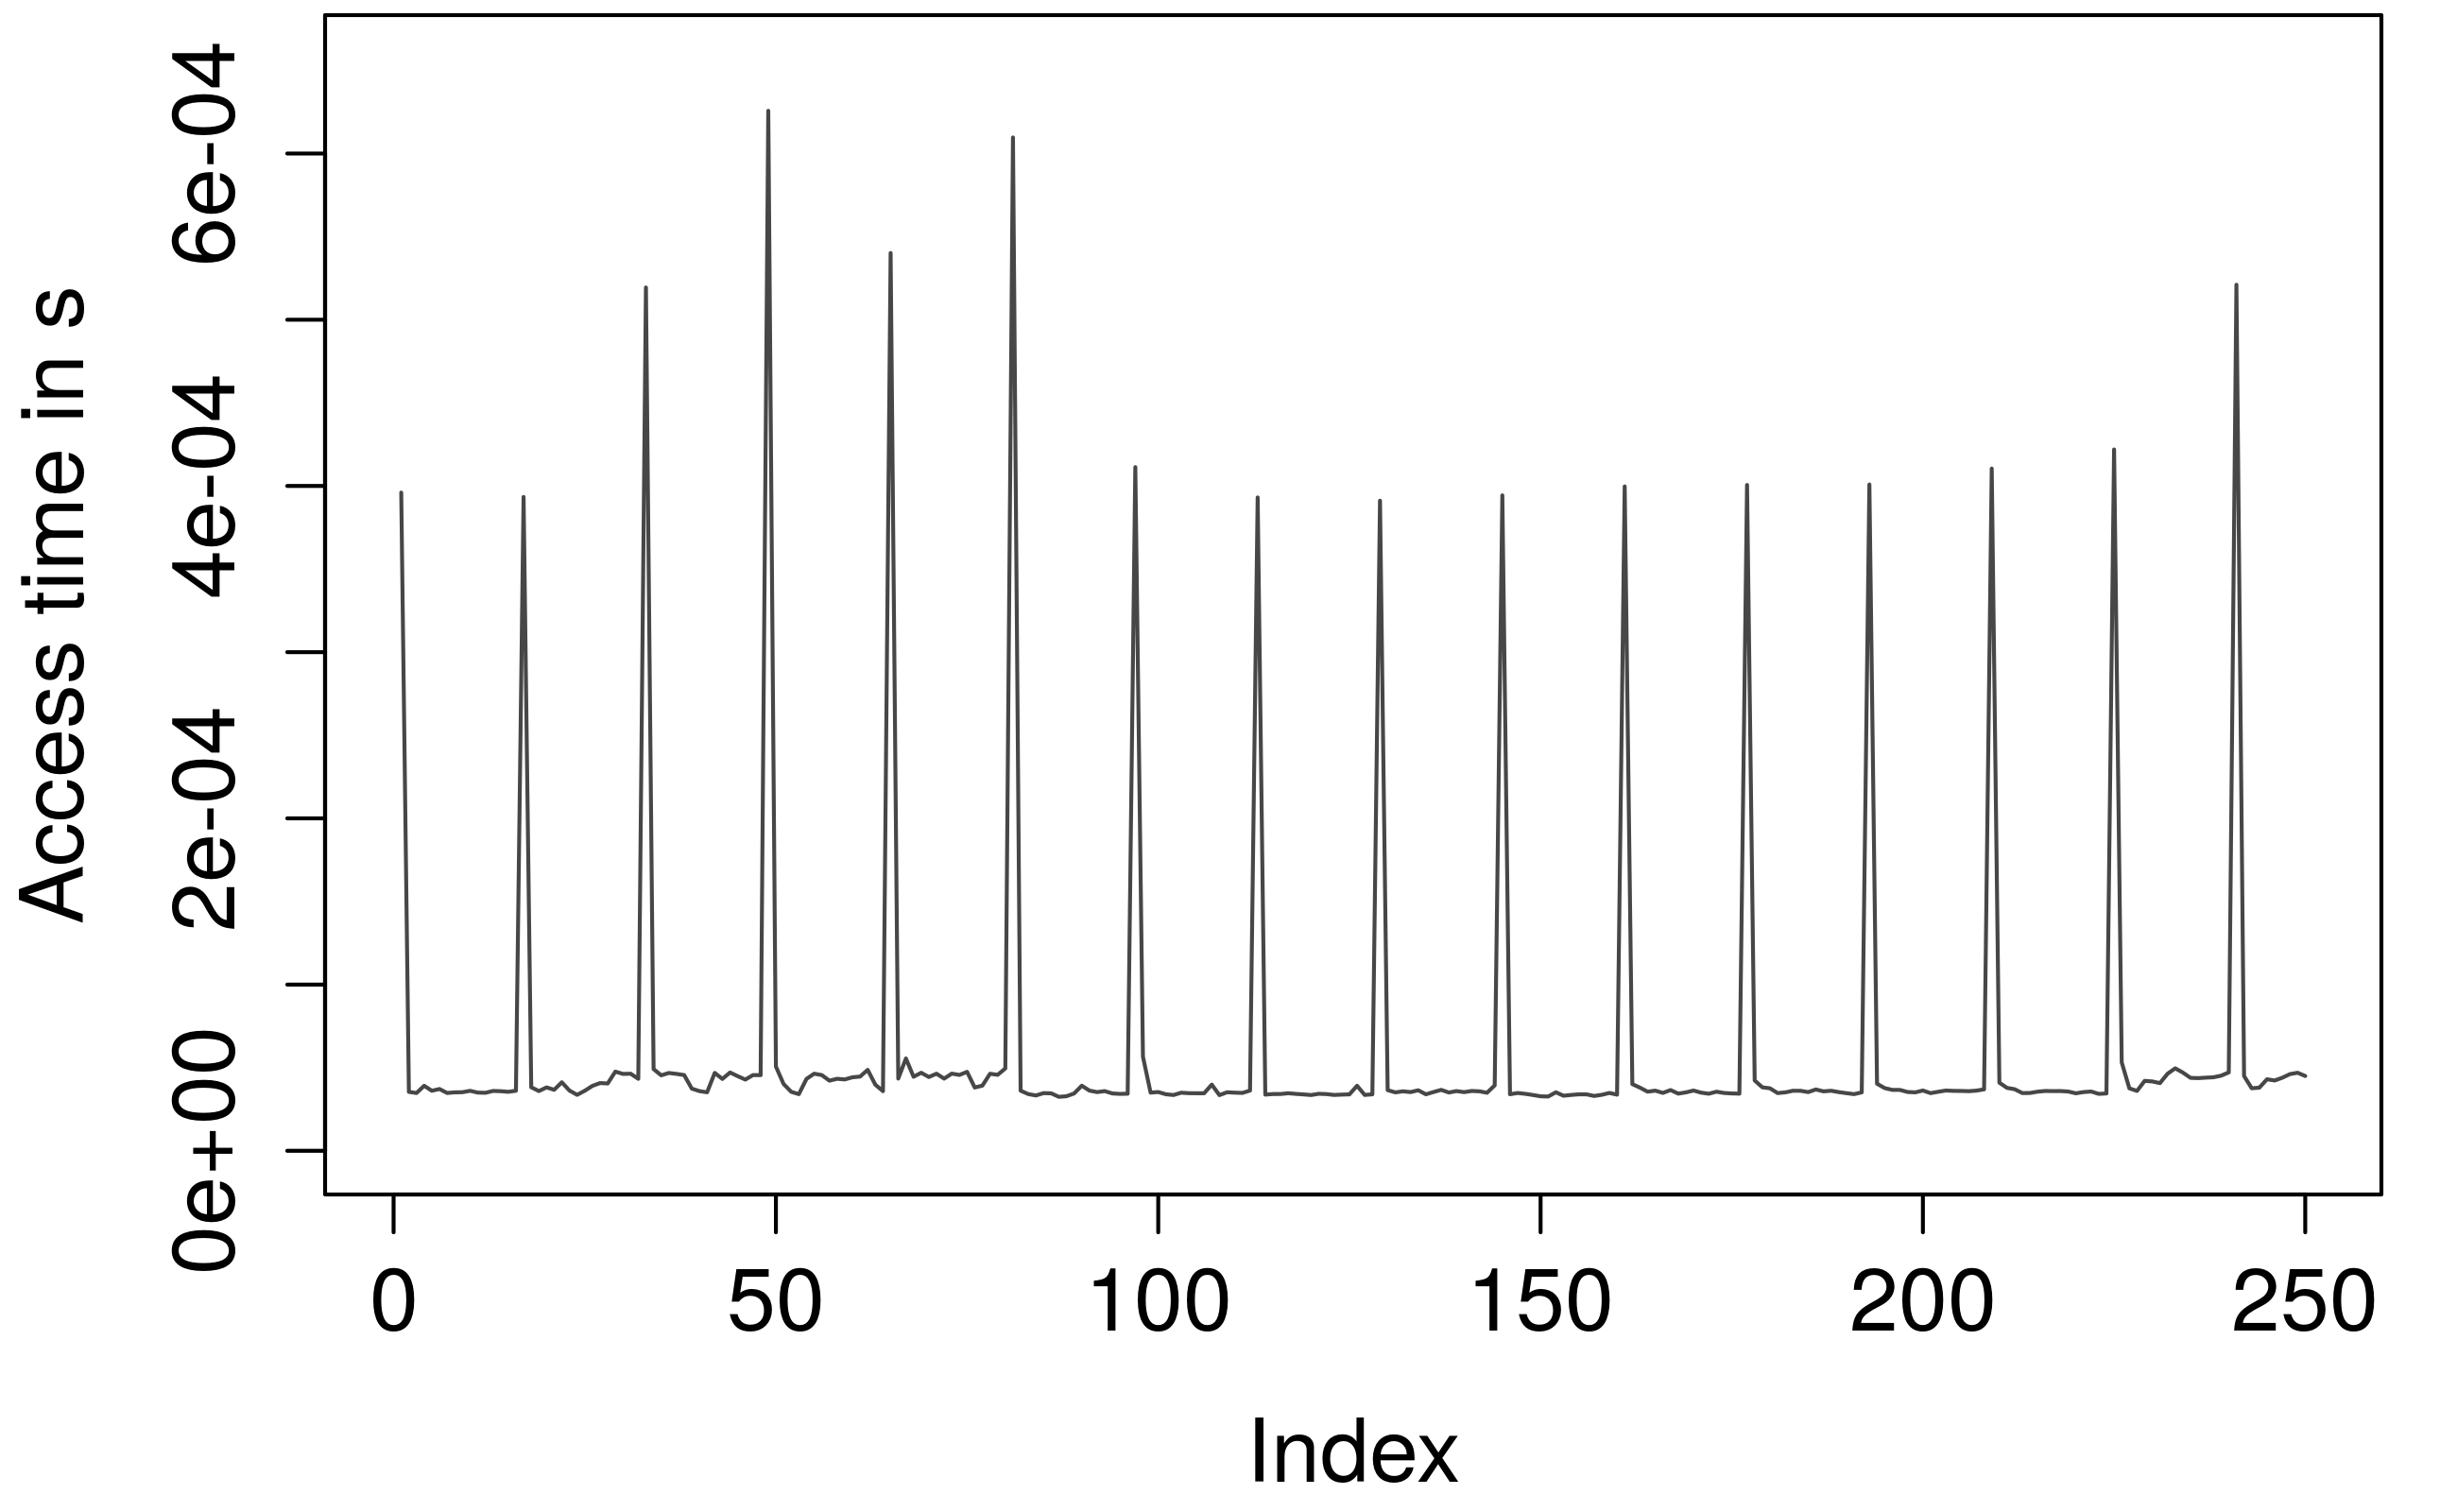
\includegraphics[width=\textwidth]{src/plot_From100001to100250_read_seq.png}
		\caption{Small sequence of reading file accesses with periodic peaks in access time.}
		\label{periodic}
	\end{minipage}
	\hfill
	\begin{minipage}[b]{0.47\textwidth}
		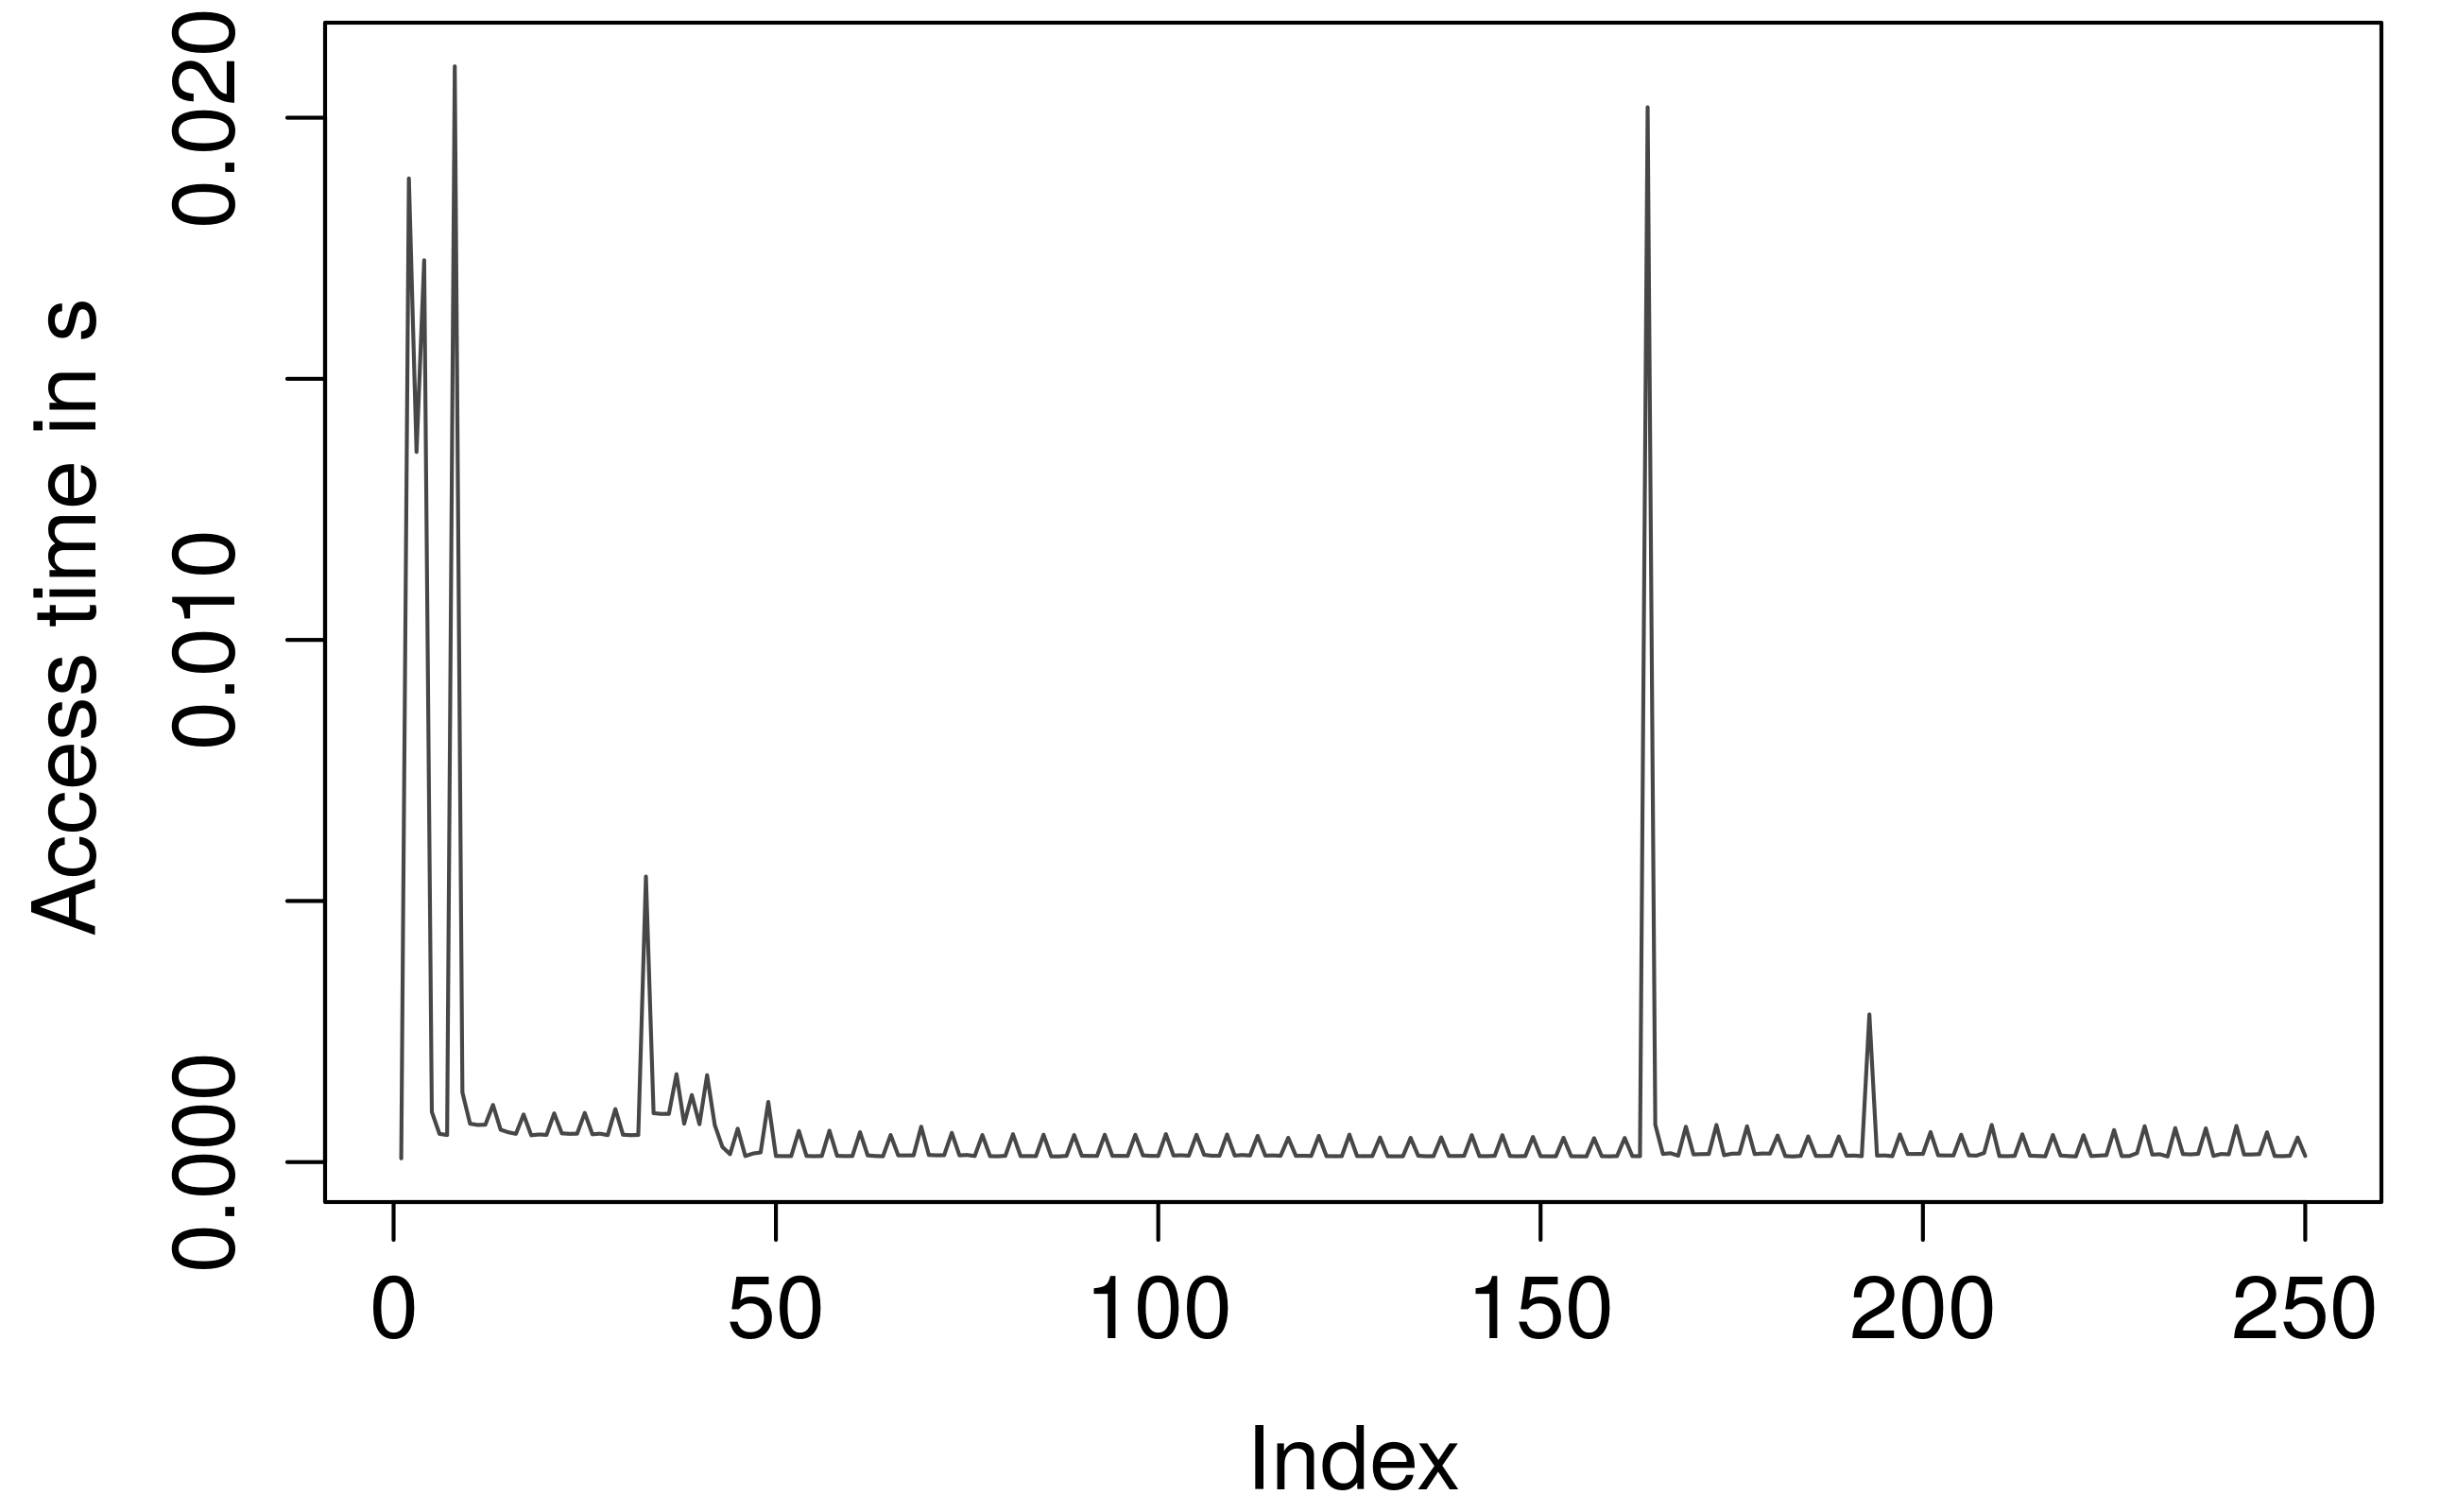
\includegraphics[width=\textwidth]{src/plot_First250_read_seq.png}
		\caption{Small sequence of reading file accesses with sporadic peaks in access time.}
		\label{sporadic}
	\end{minipage}
\end{figure}
%\fig{width=0.47\textwidth}{src/plot_From100001to100250_read_seq.png}{Small sequence of reading file accesses with periodic peaks in access time.}
%\fig{width=0.47\textwidth}{src/plot_First250_read_seq.png}{Small sequence of reading file accesses with sporadic peaks in access time.}
With knowledge about these period of peaks a model could make better access time predictions.
Our second model is supposed to use its input information of previous data throughput for that.
The data throughput has peaks the same period as the access time.
Internally the model calculates the exponential moving average (EMA) of data throughput of measurement $i$ as:
\begin{equation}
EMA(i) = 0.5 \cdot t(i)+ 0.5 \cdot EMA(i-1)
\end{equation}
With $t(i)$ the access time of measurement $i$.
The influence of data throughput of a measurement is exponentially decreasing in the series of EMAs.
In Figure \ref{src/ema2.png} the EMA-function to a graph with periodic peaks can be seen.
\fig{width=.47\textwidth}{src/ema2.png}{Exponential moving average in red for a graph with perdiodic peaks.}\\
The ema-model can use $EMA(n-1)$ for the prediction of access time of measurement $n$.
If the model is able to find threshold values of the EMA-function after which another peaks follows, it can use this input information for better access time predictions on sequences with periodic peaks in access time. Depending on how relevant periodic behavior of access times is in our measurements, this additional input information could improve the model.\medskip

The error-class-model is used as described in Section\,\ref{sec:error_classes} to examine the potential improvements for access time prediction due to knowledge about I/O-paths.
Therefore, we evaluate how much the prediction of access times of a model using error classes improves compared to a model without.

\section{Evaluation}
\label{evaluation}
The execution and results of analysis are summarized in the following.
First the test system used for measurements and the strategy for systematic measurement are presented.
Then follows the study of received data and computed error classes.
And in the end the quality of predictions of the different models are examined.

\subsection{Test system}
The measurements were done on the super computer Mistral of the DKRZ (Deutsches Klimarechenzentrum).
Mistral operates with the parallel distributed file system Lustre (Lustre 2.5, Seagate's edition) and consists of over 1500 computing nodes and 30 petabyte storage with a memory bandwidth of 300\,GiB/s.
Each computing node consists of two E5-2680v3 with a clock rate of 2.5\,GHz and 30\,MiB L3 Cache.
Measurements were done during daily operation, typical fluctuations in workload may have influenced the execution of benchmarks.

\subsection{Benchmarking}
We created a simple benchmark (io-model) that used POSIX read/write() and measured time for each I/O individually.
In this paper, it is executed on one node with one processor to study the quality of the predictions.
Each series of measurements follows a certain pattern to study system behavior systematically.\\
Sequential and random I/O patterns are measured, each with reading and writing file accesses.
Our test file has a size of 10\,GiB which doesn't fit in the main memory of computer nodes, also measurements from  suggest that caching is not effective for these measurements (sequential reads are improved by read-ahead, though).
Occasional access of hard drives in the parallel storage system is likely.
Most series of measurements contain 10\,000 file accesses with a certain access size, only series with sequential access and an access size of greater then 2\,MiB have fewer measurements as the end of our 10\,GiB file is reached.
Every series with specific access pattern, access size and access type is repeated three times.
Access sizes are varying from 1\,B to 16\,MiB (in detail:  1\,B, 4\,B, 16\,B, 64\,B, 256\,B, 1\,KiB, 4\,KiB, 8\,KiB, 16\,KiB, 64\,KiB, 256\,KiB, 512\,KiB, 1\,MiB, 2\,MiB, 4\,MiB, 8\,MiB and 16\,MiB).

\subsection{Analysis of measurements}
\label{sec:measurements}
At first the measured access times for the four different cases are summarized in Table\,\ref{overview}.
\tab{overview}{Overview of file access times for the different cases.}{
	\centering
	\scriptsize
	\begin{tabular}{|r|r|r|r|r|r|r|}\hline%
		Case & Min. value  & 1. Quartile & Median & Arith. mean & 3. Quartile & Max. value \\\hline\hline
		\csvreader[late after line=\\\hline]%
		{src/data_summary.csv}{Attribut=\Attribut,Min=\Min,Quartil1=\L, Median = \Median, Mittel = \Mittel,Quartil3 = \Q, Max = \Max, Korrelation = \Korrelation}%
		{\Attribut & \Min & \L & \Median & \Mittel & \Q & \Max}%
	\end{tabular}
}\\
As expected, sequential file accesses are on average much faster than random accesses especially for the reading case, also random read are slower than writes.\\
In Figure \ref{correlations}, we consider the correlations between file access parameters and the resulting access time, a strong correlation can be exploited for access time prediction.
\tab{correlations}{Correlations between file access parameters and access time.}{
	\centering
	\scriptsize
	\begin{tabular}{|r|r|r|}\hline%
		Attribute & Sequential access pattern & Random access pattern\\\hline\hline
		\csvreader[late after line=\\\hline]%
		{src/data_summary_korrelationen.csv}{Attribut=\Attribut,seq = \seq, rnd = \rnd}%
		{\Attribut & \seq &\rnd}%
	\end{tabular}
}\\
It is to note that sequential access leads to a constant delta-offset of $0$.
Sequential file accesses have with 97.3\% a clear correlation to access time, this is with only 32.91\% to a lesser degree still true for the random accesses.
This is why linear regression can be expected to have acceptable results for access time prediction, especially for the sequential access case.\medskip

To study the distribution of measured file access times we display them as follows:
All measurements with equal access size have the same color, access sizes of file accesses are increasing in the graphs from left to right.
The resulting graphs can be seen in the Figures \ref{read_seq} to \ref{write_rnd}.

\begin{figure}[!h]
	\centering
	\begin{minipage}[b]{0.47\textwidth}
		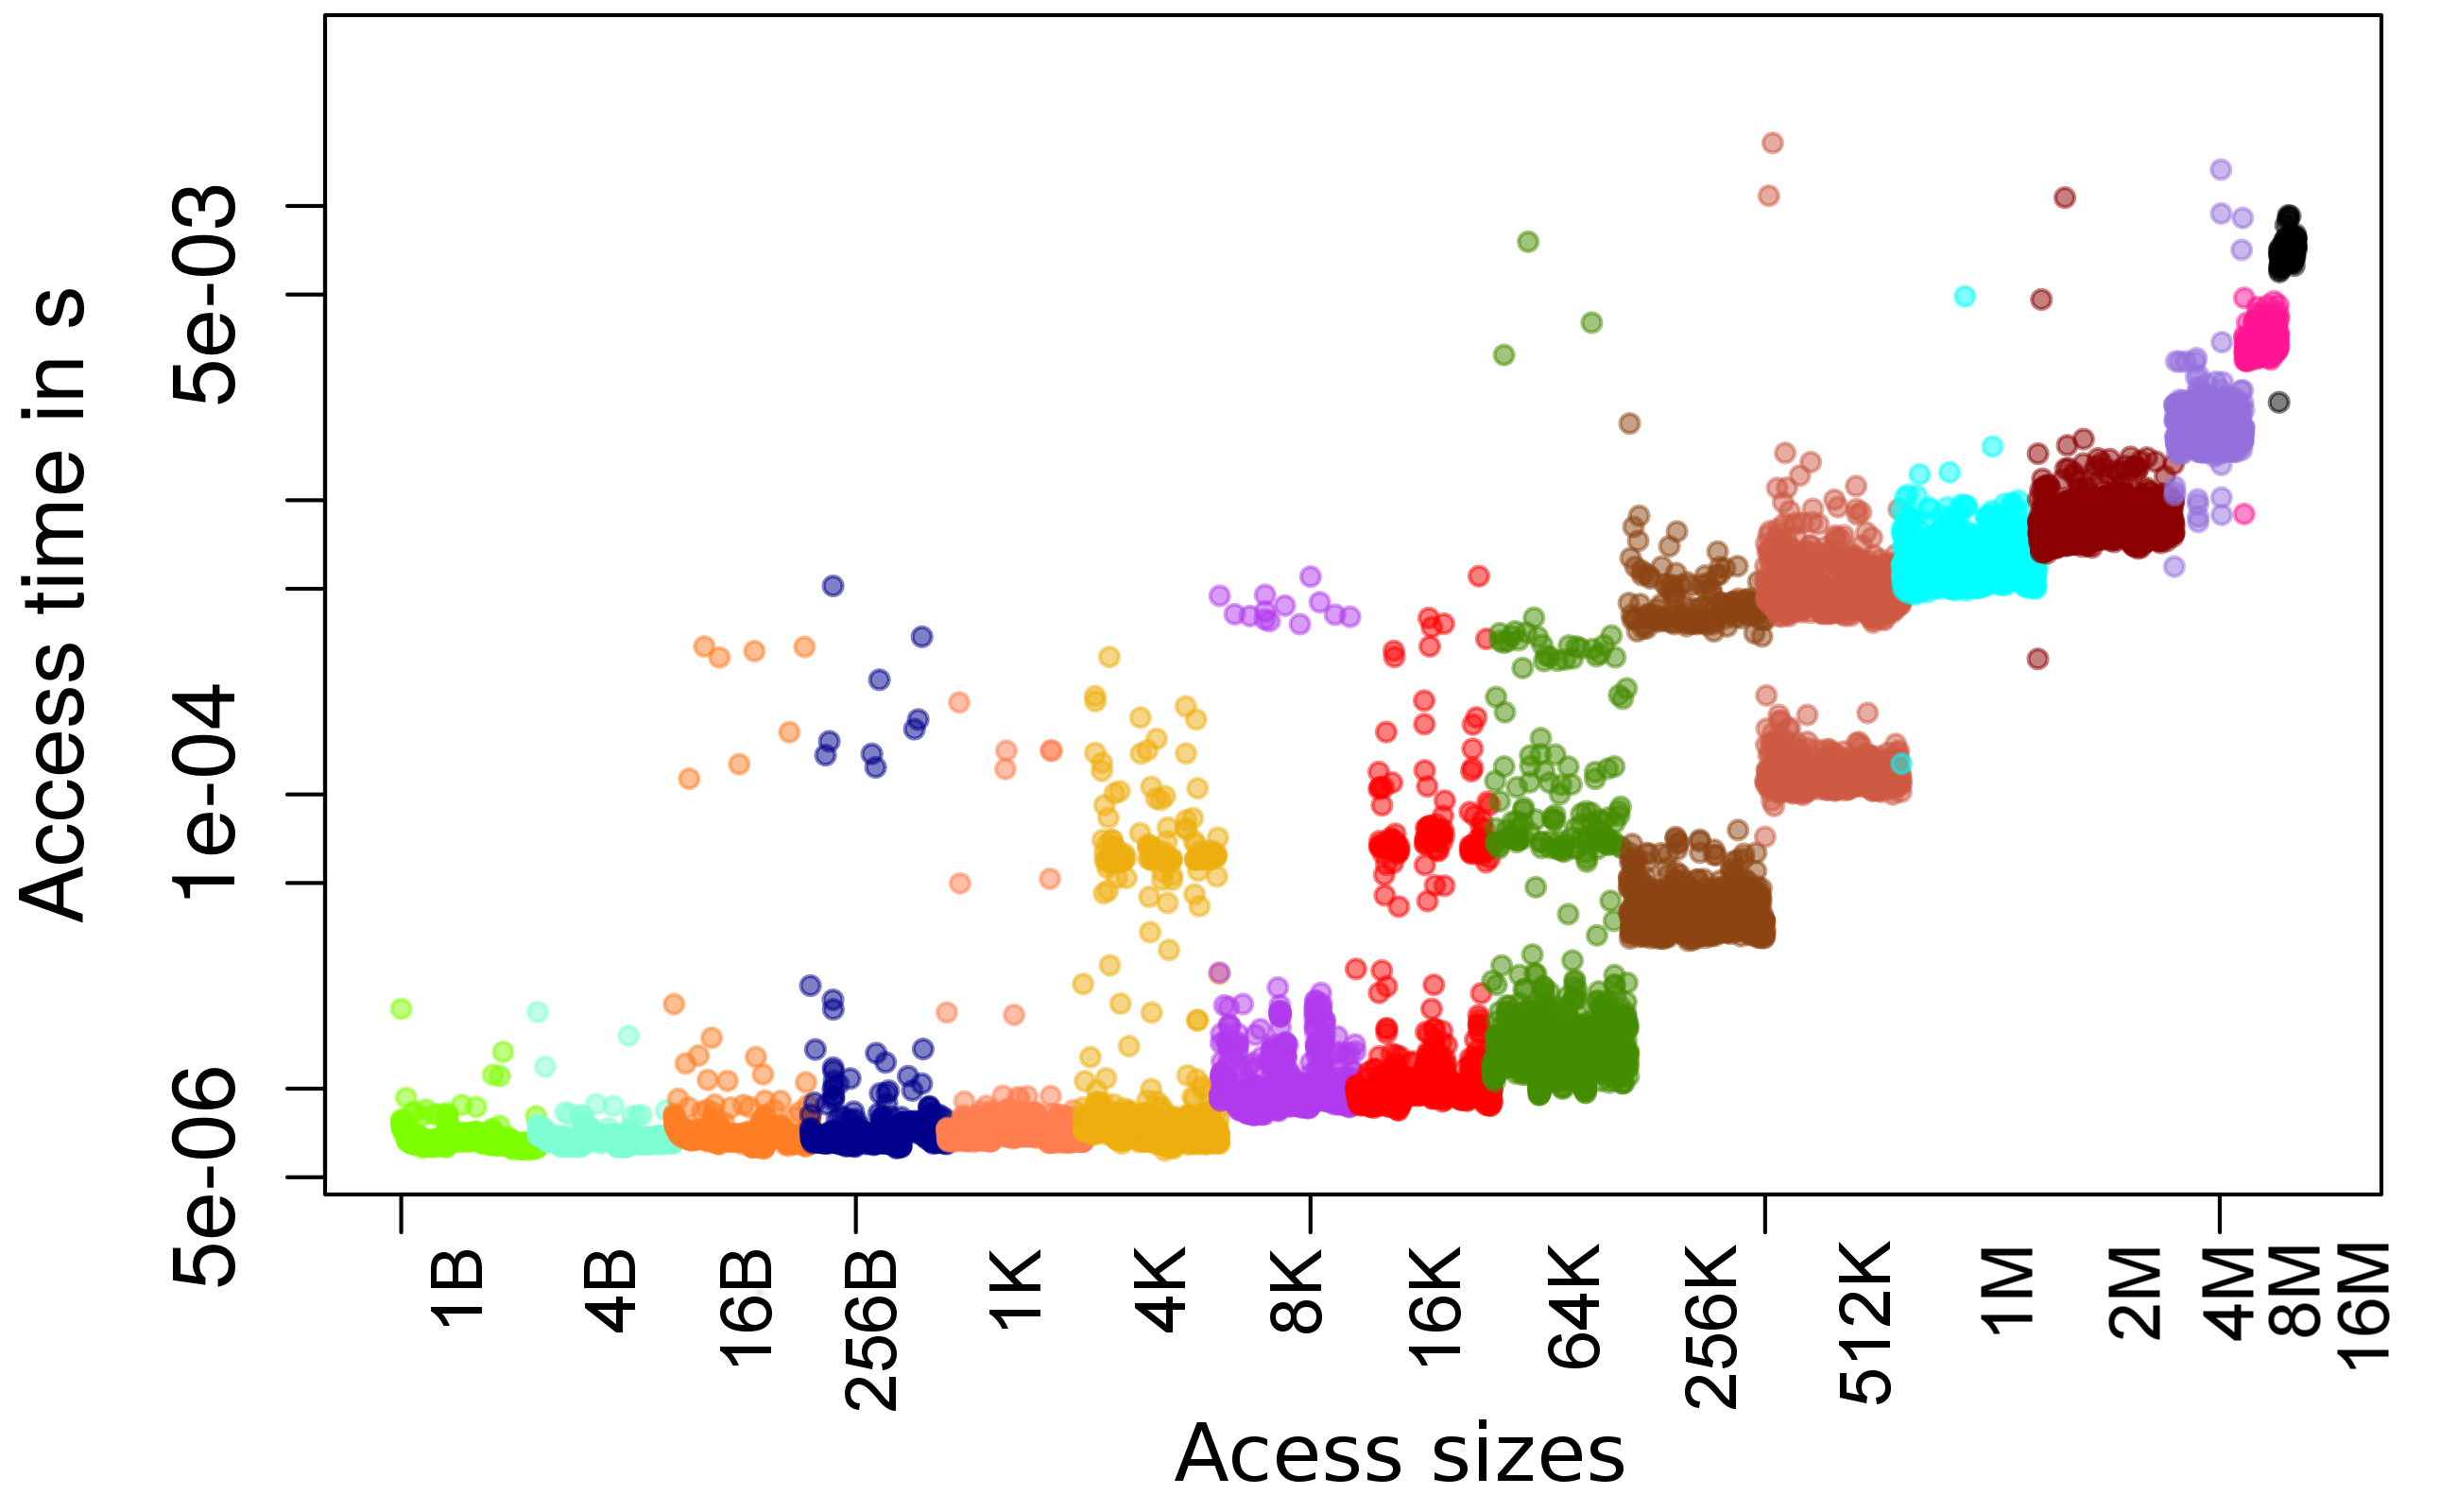
\includegraphics[width=\textwidth]{src/plot_SizeSorted_log_read_seq2.png}
		\caption{Measurements of sequential reading file accesses.}
		\label{read_seq}
	\end{minipage}
	\hfill
	\begin{minipage}[b]{0.47\textwidth}
		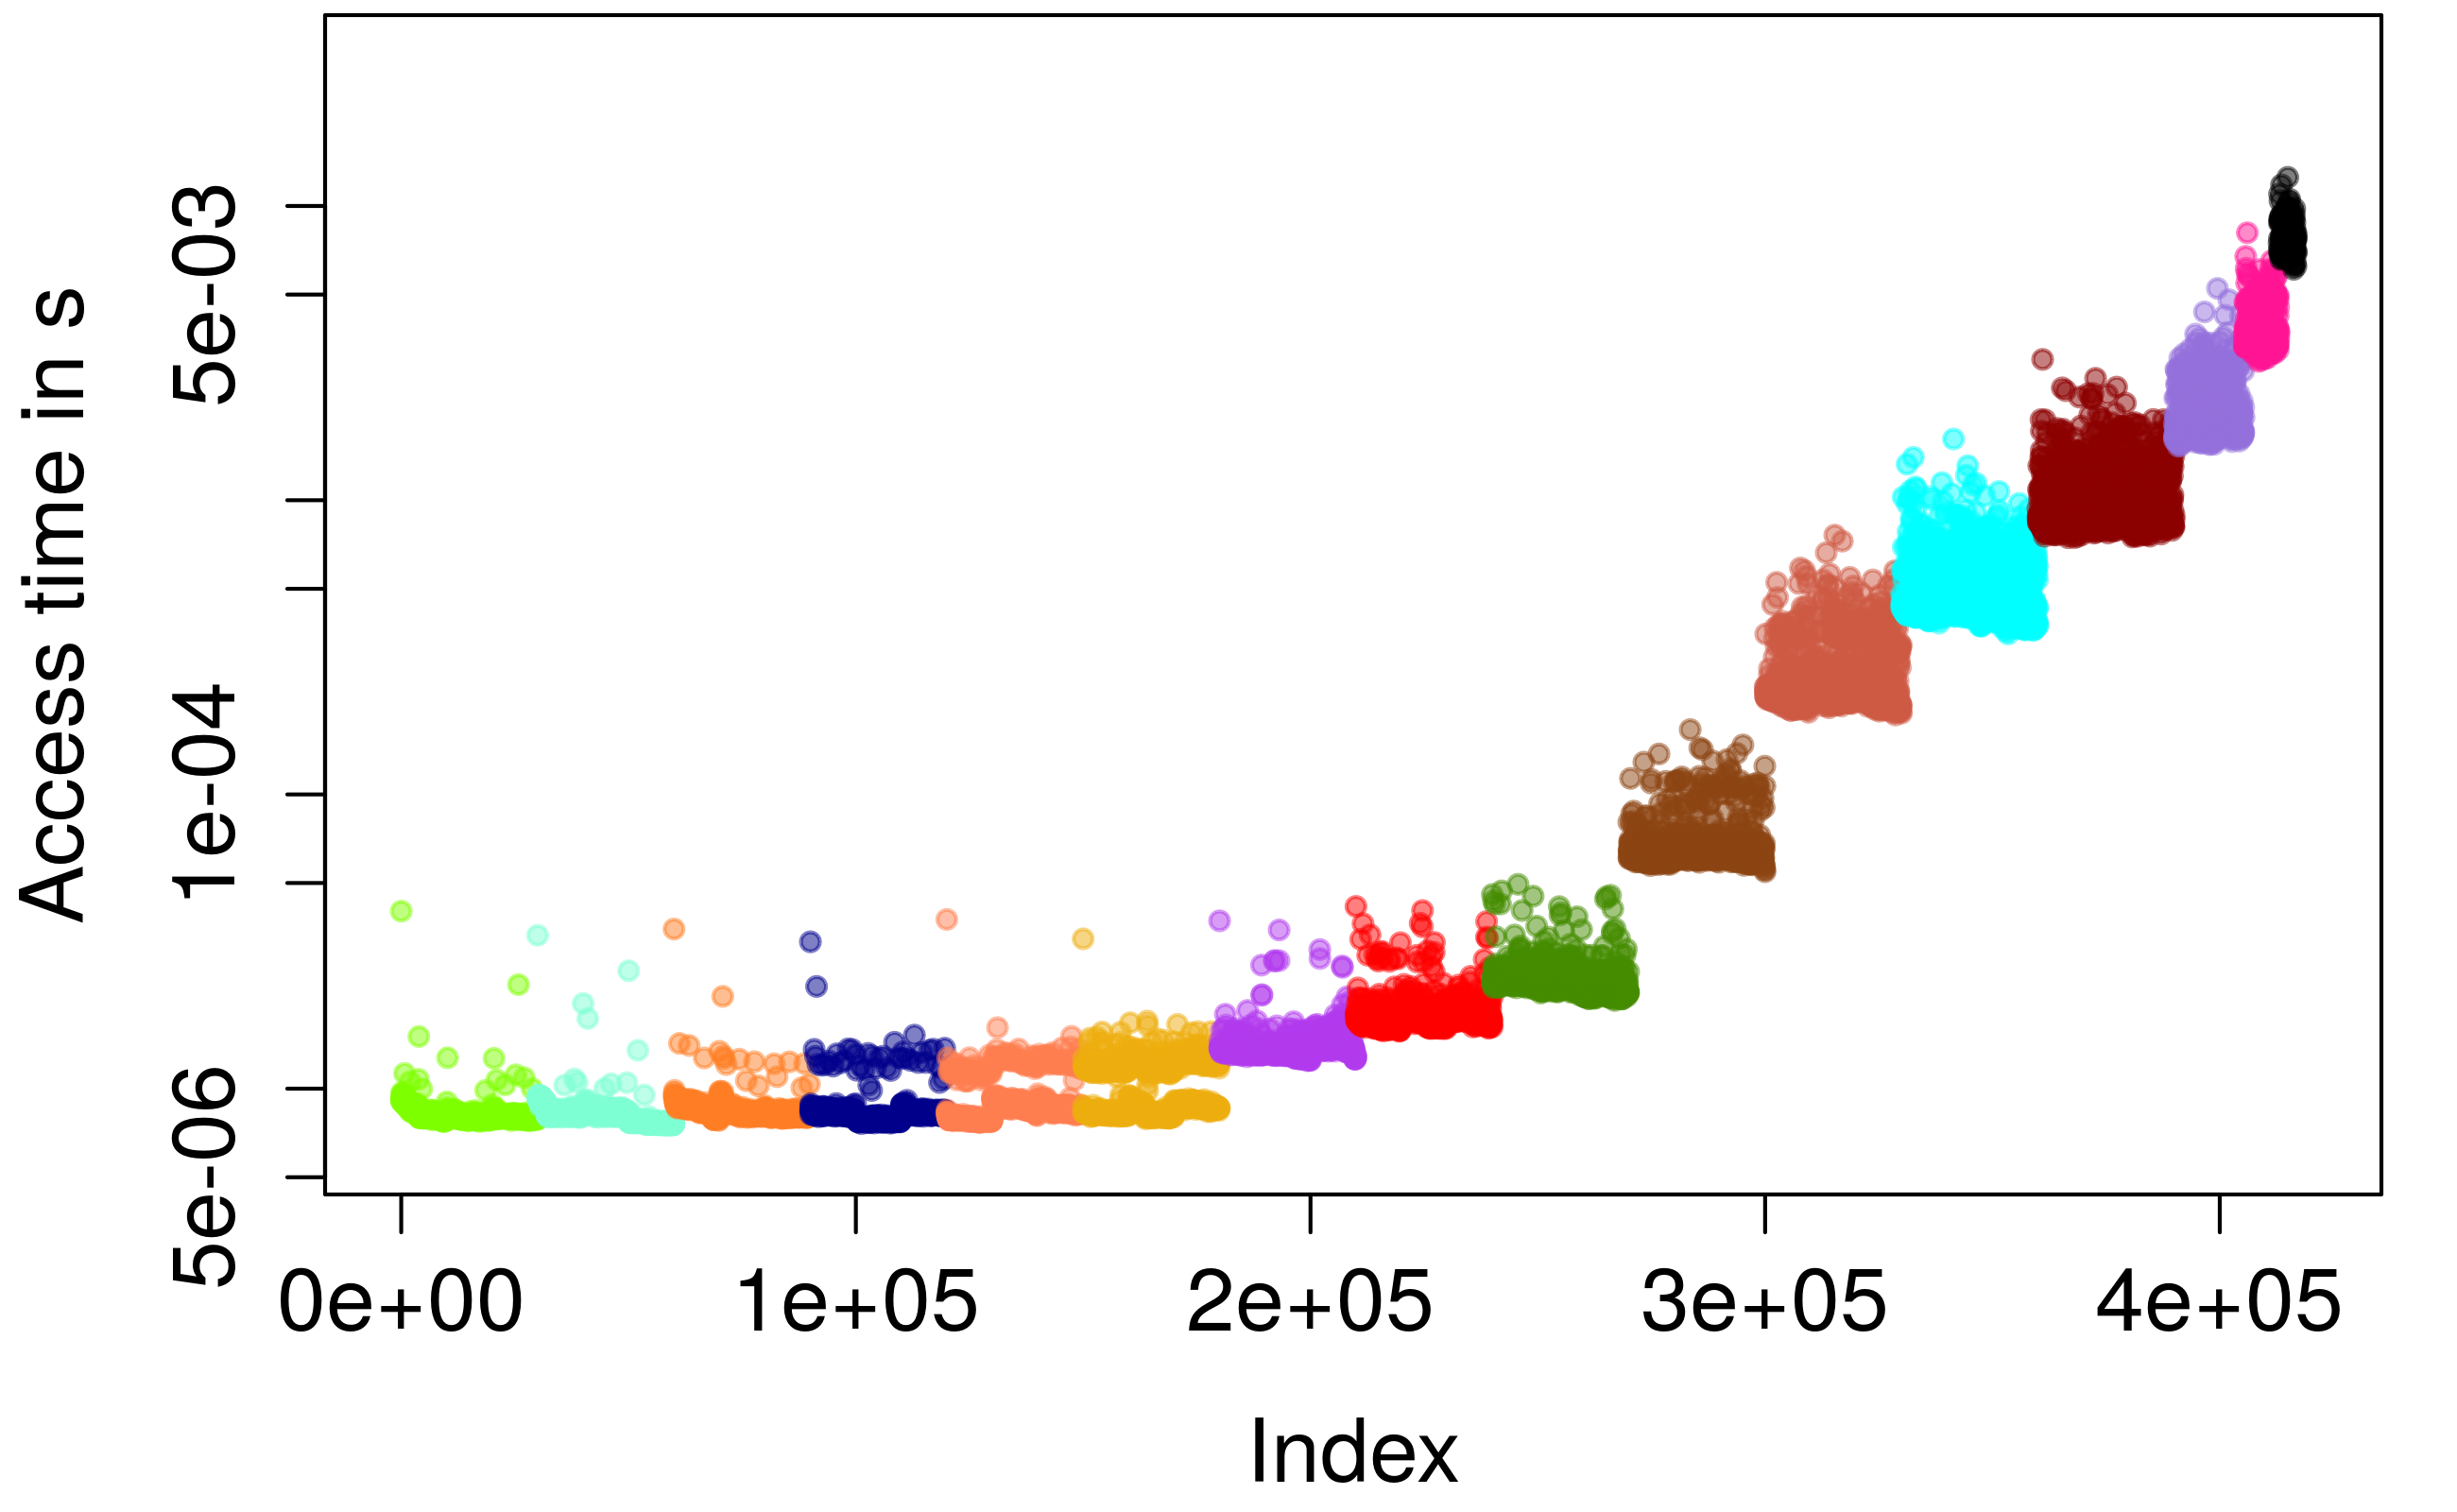
\includegraphics[width=\textwidth]{src/plot_SizeSorted_log_write_seq.png}
		\caption{Measurements of sequential writing file accesses.}
		\label{write_seq}
	\end{minipage}
\end{figure}
\begin{figure}[!h]
	\centering
	\begin{minipage}[b]{0.47\textwidth}
		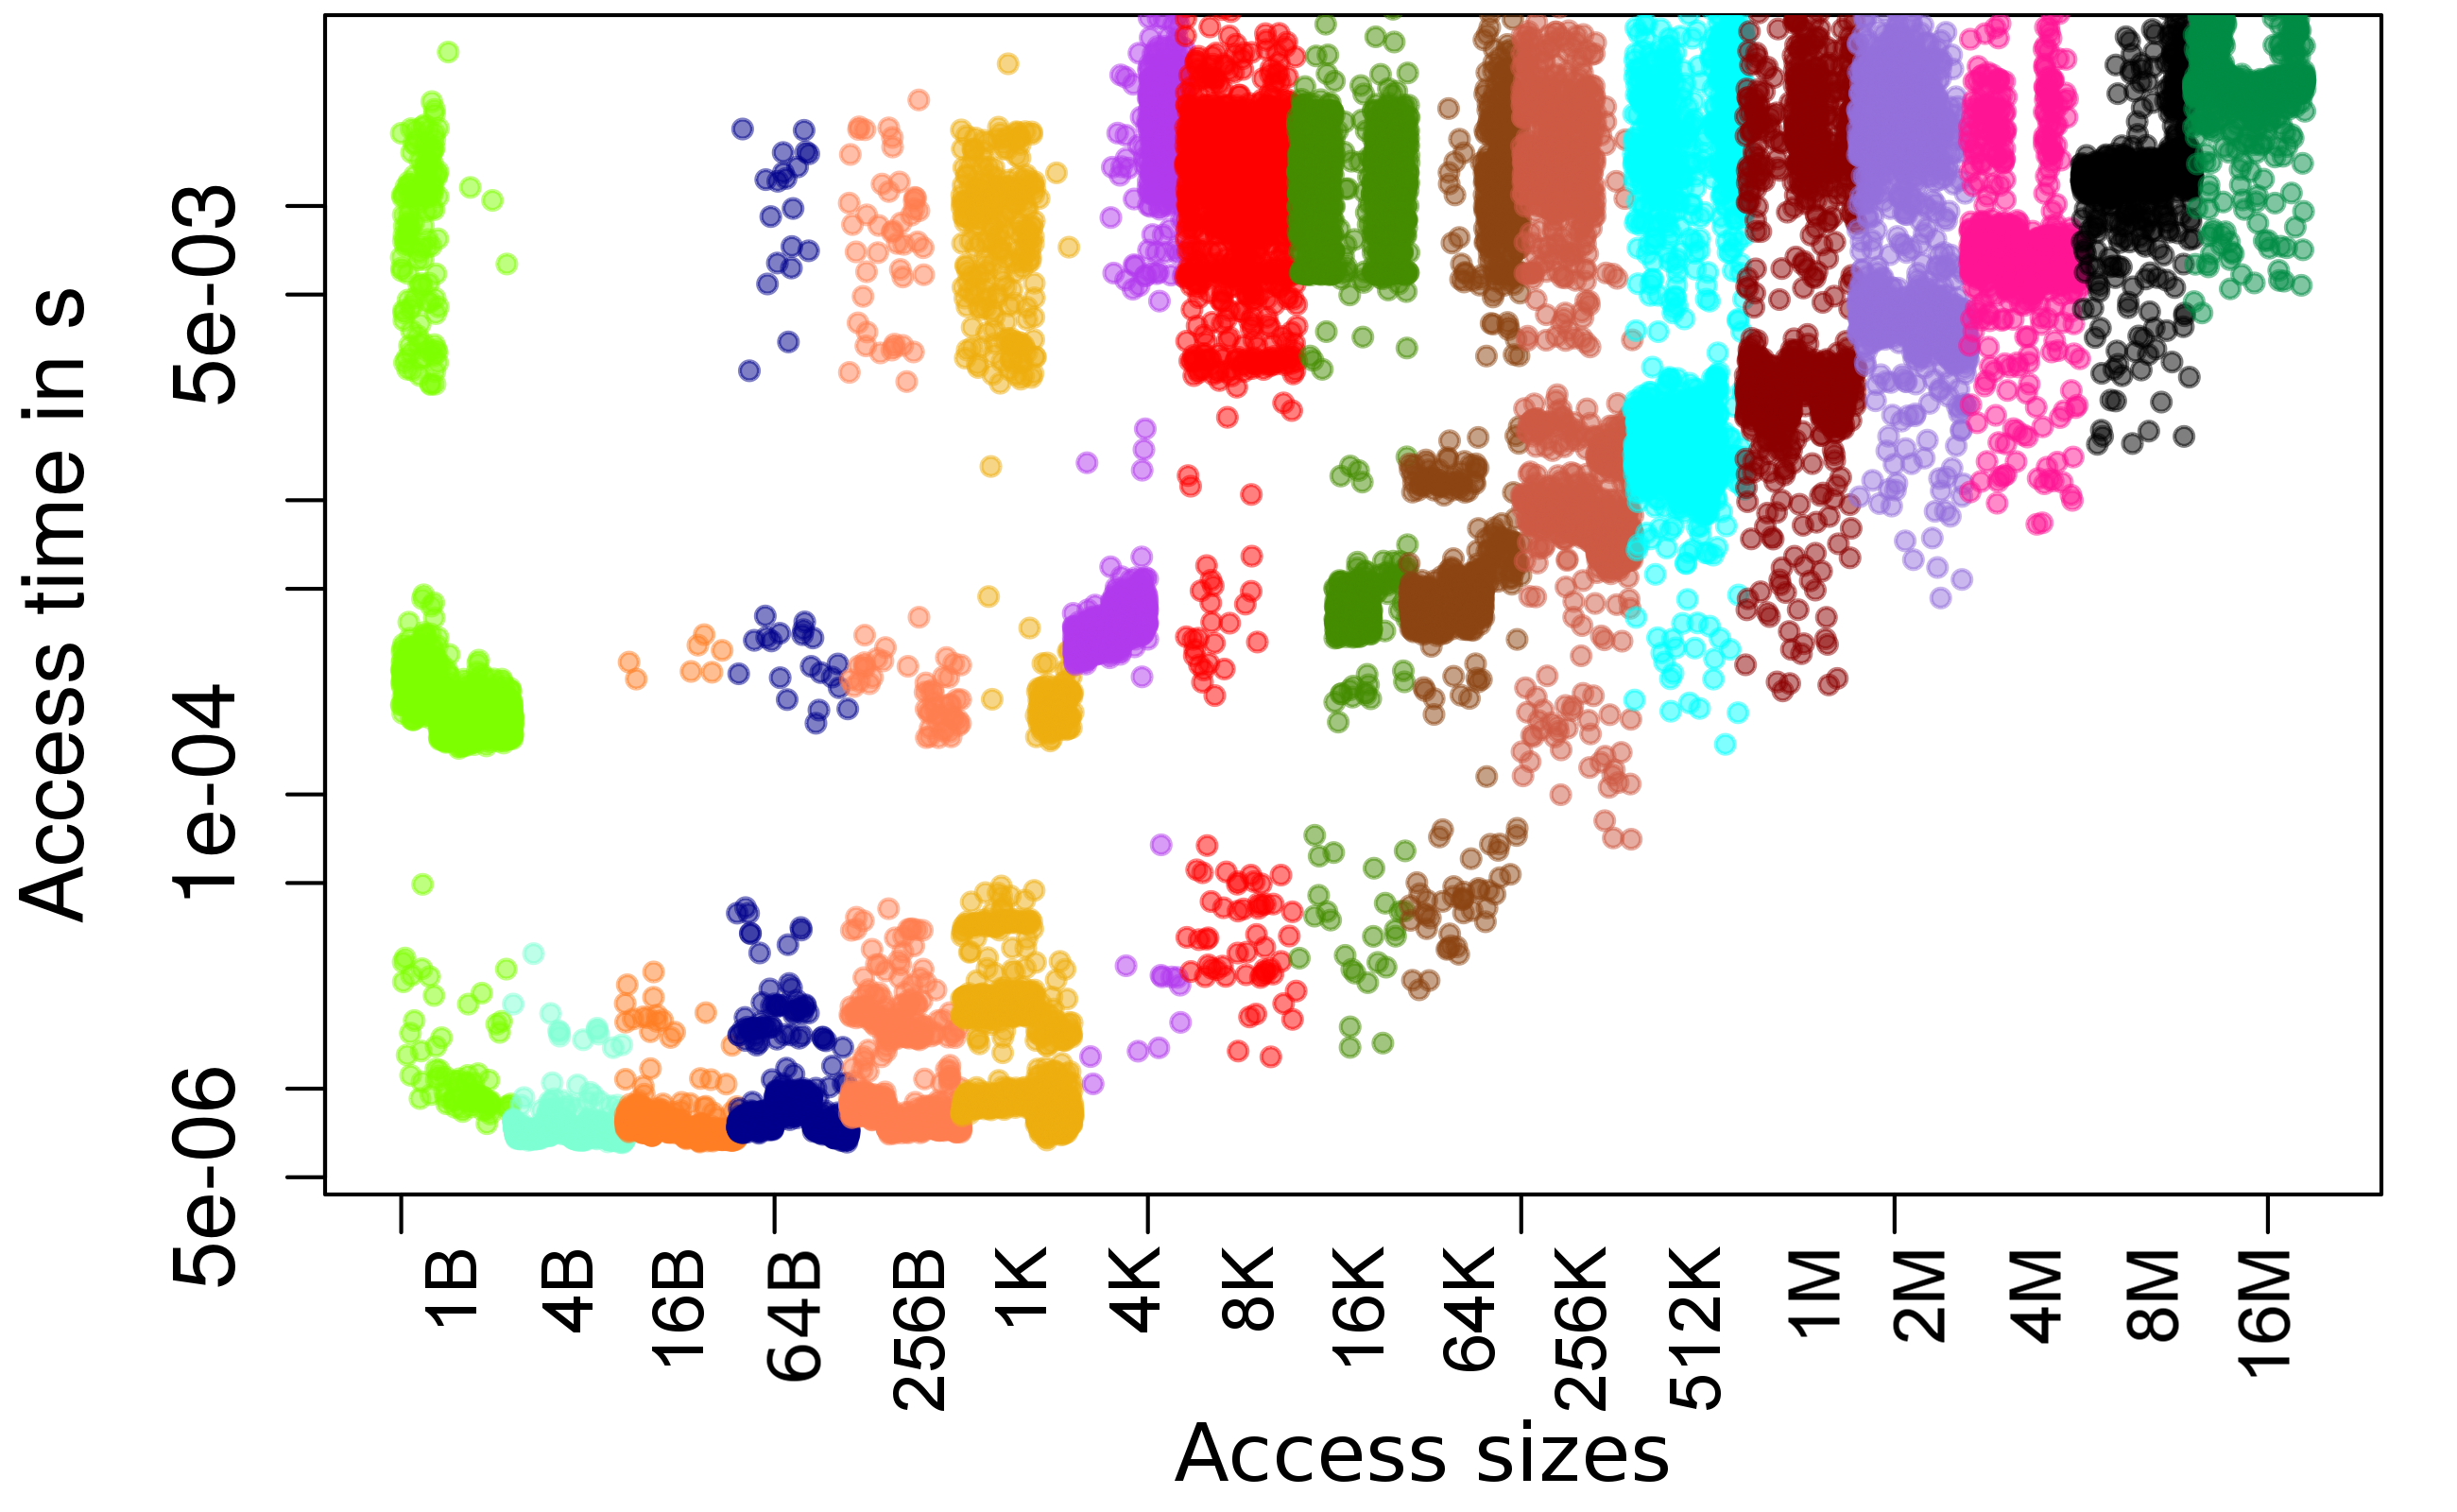
\includegraphics[width=\textwidth]{src/plot_SizeSorted_log_read_rnd.png}
		\caption{Measurements of random reading file accesses.}
		\label{read_rnd}
	\end{minipage}
	\hfill
	\begin{minipage}[b]{0.47\textwidth}
		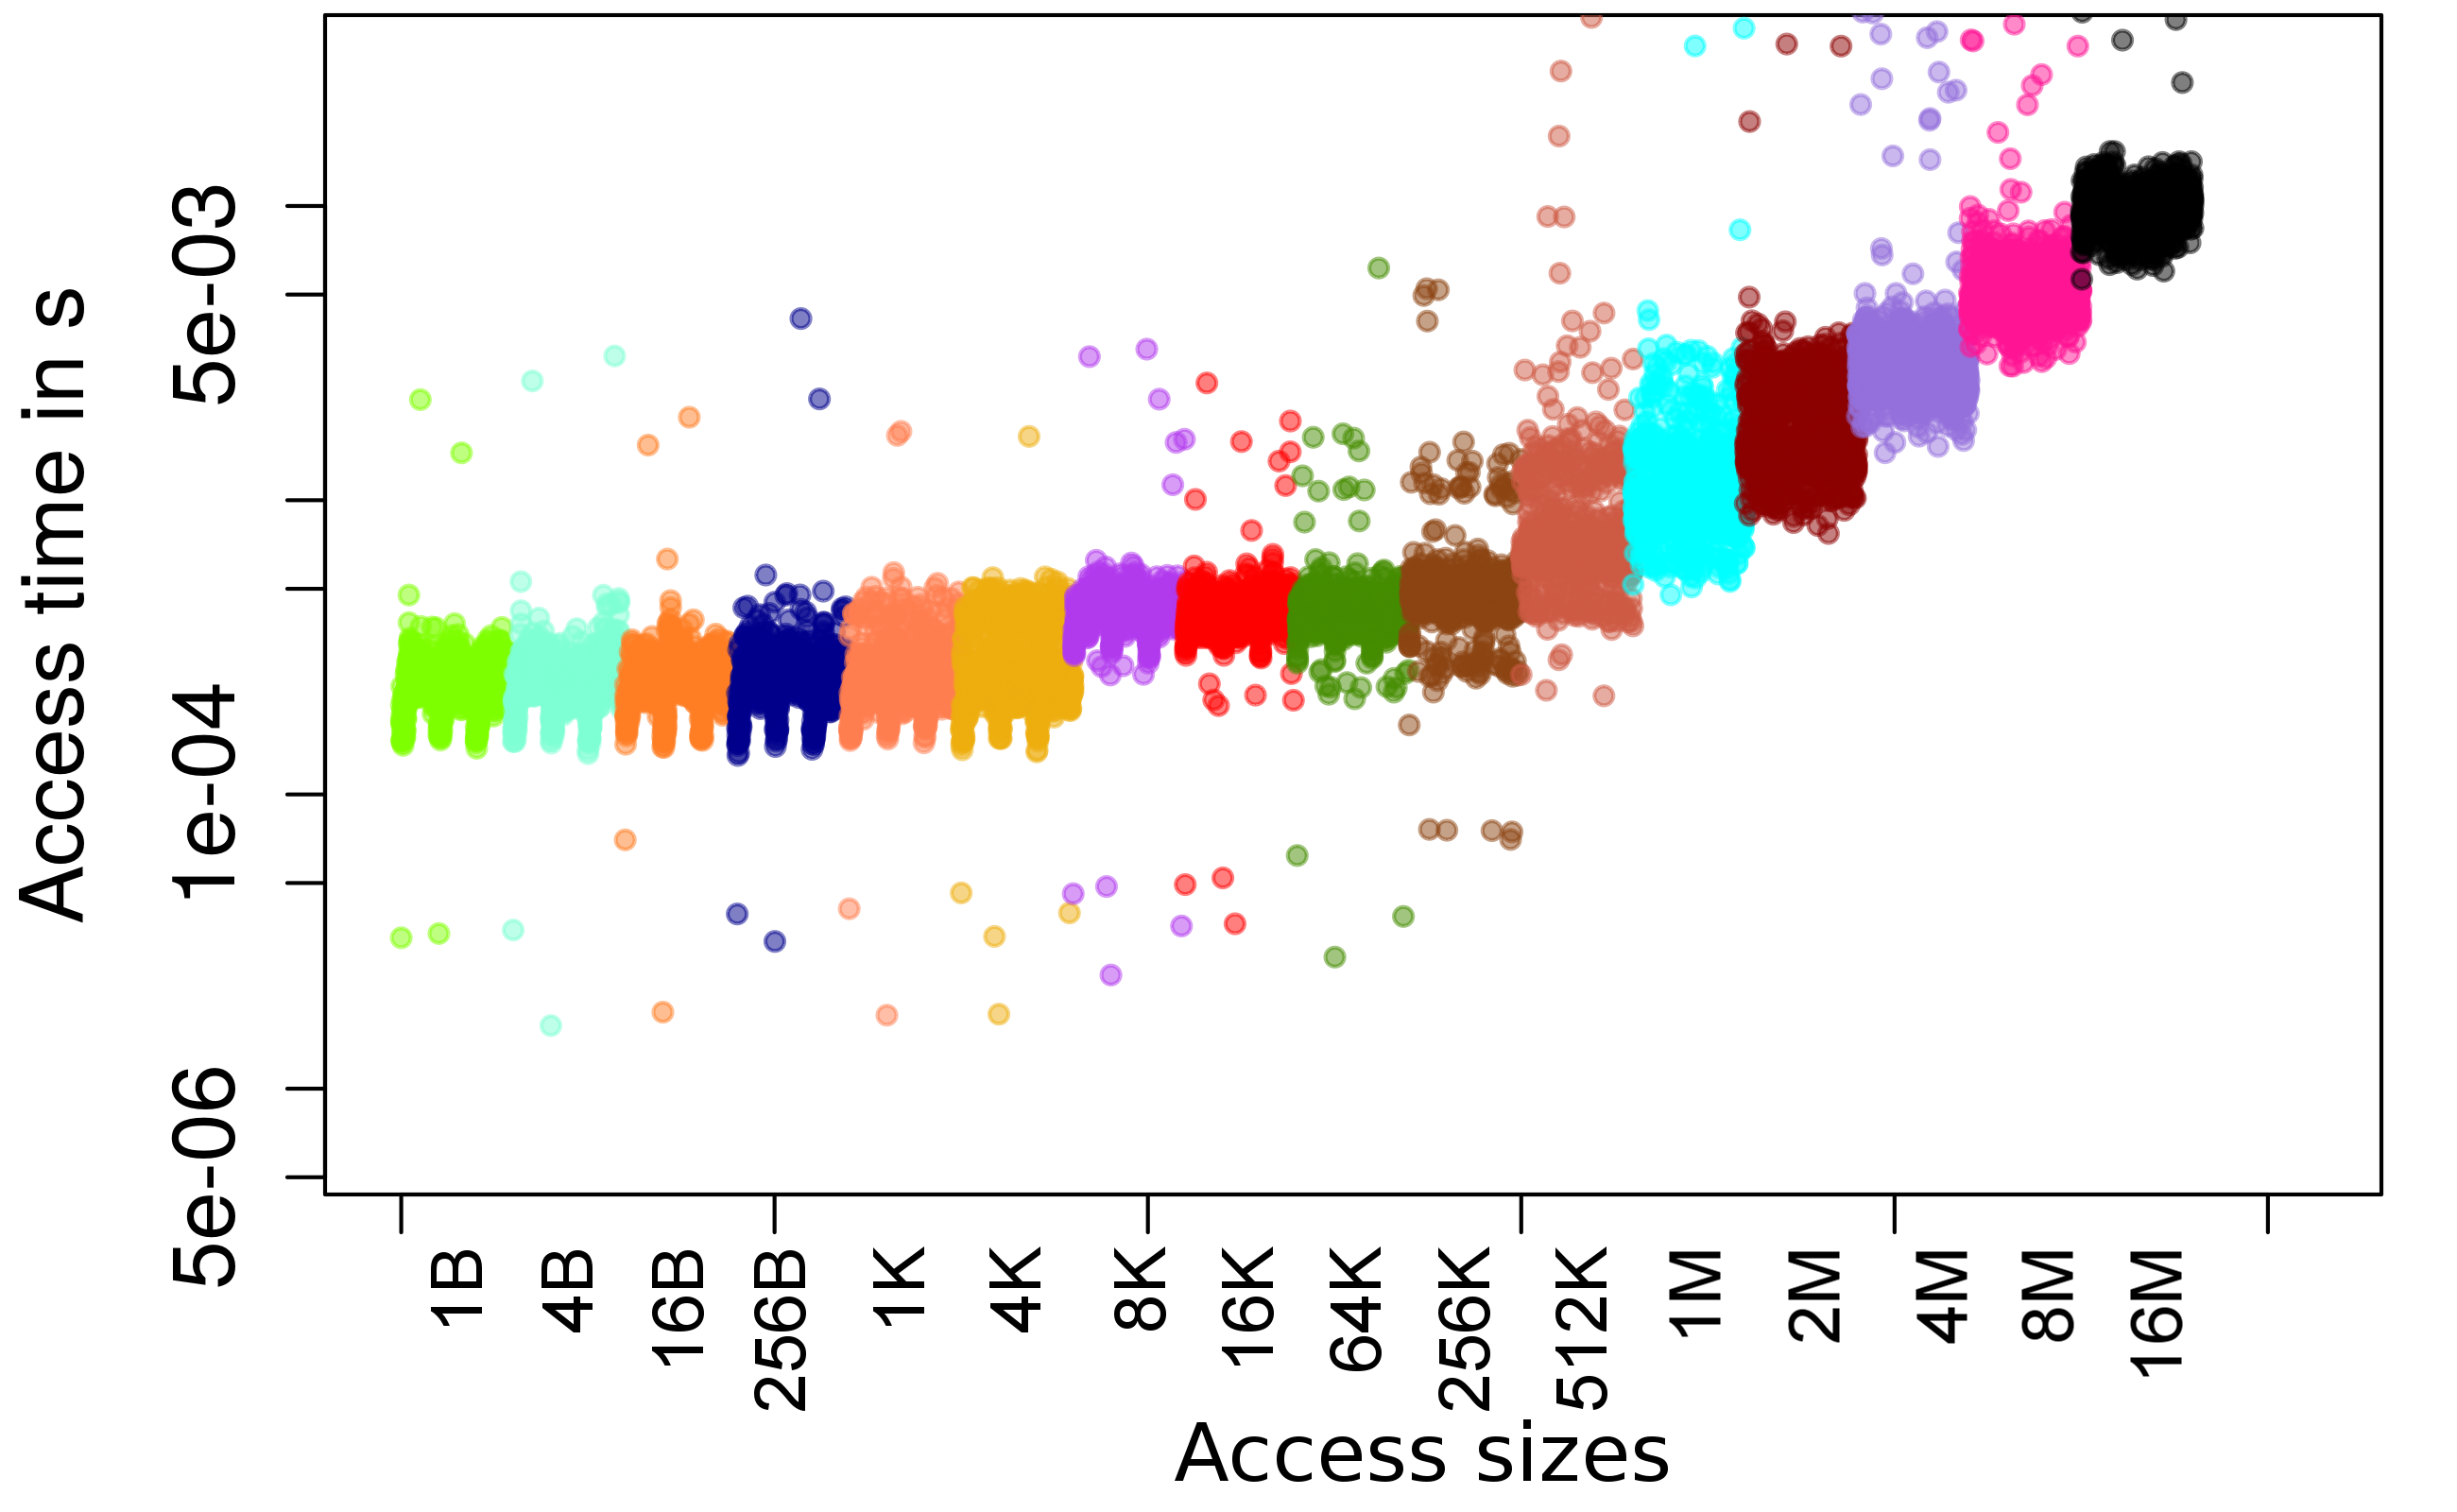
\includegraphics[width=\textwidth]{src/plot_SizeSorted_log_write_rnd.png}
		\caption{Measurements of random writing file accesses.}
		\label{write_rnd}
	\end{minipage}
\end{figure}

%\fig{width=.47\textwidth}{src/plot_SizeSorted_log_read_seq2.png}{Measurements of sequential reading file accesses.}
%\fig{width=.47\textwidth}{src/plot_SizeSorted_log_write_seq.png}{Measurements of sequential writing file accesses.}
%\fig{width=.47\textwidth}{src/plot_SizeSorted_log_read_rnd.png}{Measurements of random reading file accesses.}
%\fig{width=.47\textwidth}{src/plot_SizeSorted_log_write_rnd.png}{Measurements of random writing file accesses.}
For clarity the slowest and fastest 1\% of measurements are cut and only every 25th measurement is represented.\\
The correlation between access size and access time can be easily identified.
As described in chapter \ref{sec:path_for_pred} the split of measurements with equal access parameter values, that occurs in particular in the cases of sequential file accesses, can be explained with a processing in the storage system along different I/O-paths.
Worth mentioning is that the groups of access time for different access sizes are partially at the same range of magnitude.
This indicates as well that the splits are caused by varying I/O-paths as one I/O-path has a typical access time, which only changes slightly for different access sizes.\\
The phenomenon of these splits clarifies why despite of the strong correlation of access size to access time a linear model might produce sub-optimal predictions. It's difficult to predict which I/O-path will be used for a measurement as they differentiate for equal access parameter values.
In Figure \ref{read_rnd} the importance of knowledge about I/O-paths for the  access time prediction can be seen, for example file accesses of only 1\,B can be processed as slow as accesses with 16\,MiB if the longest I/O-path is used.\\
For writing file accesses the splits only occur occasionally and are less drastic; these measurements might be well represented with a linear model.

\subsection{Analysis of error classes}
Error classes are calculated as clusters of a k-means algorithm applied on the residues of the linear regression model.
As an estimation of possible I/O-paths, we classify into 10 clusters.
In Figure \ref{linreg} the predictions of linear regression on the random reading measurements can be seen as blue points.
Since a linear model predicts the mean value for all measurements with the same arguments, it cannot distinguish between the different I/O path and may not even predict a valid value (e.g., the median).

\begin{figure}[!h]
	\centering
	\begin{minipage}[b]{0.47\textwidth}
		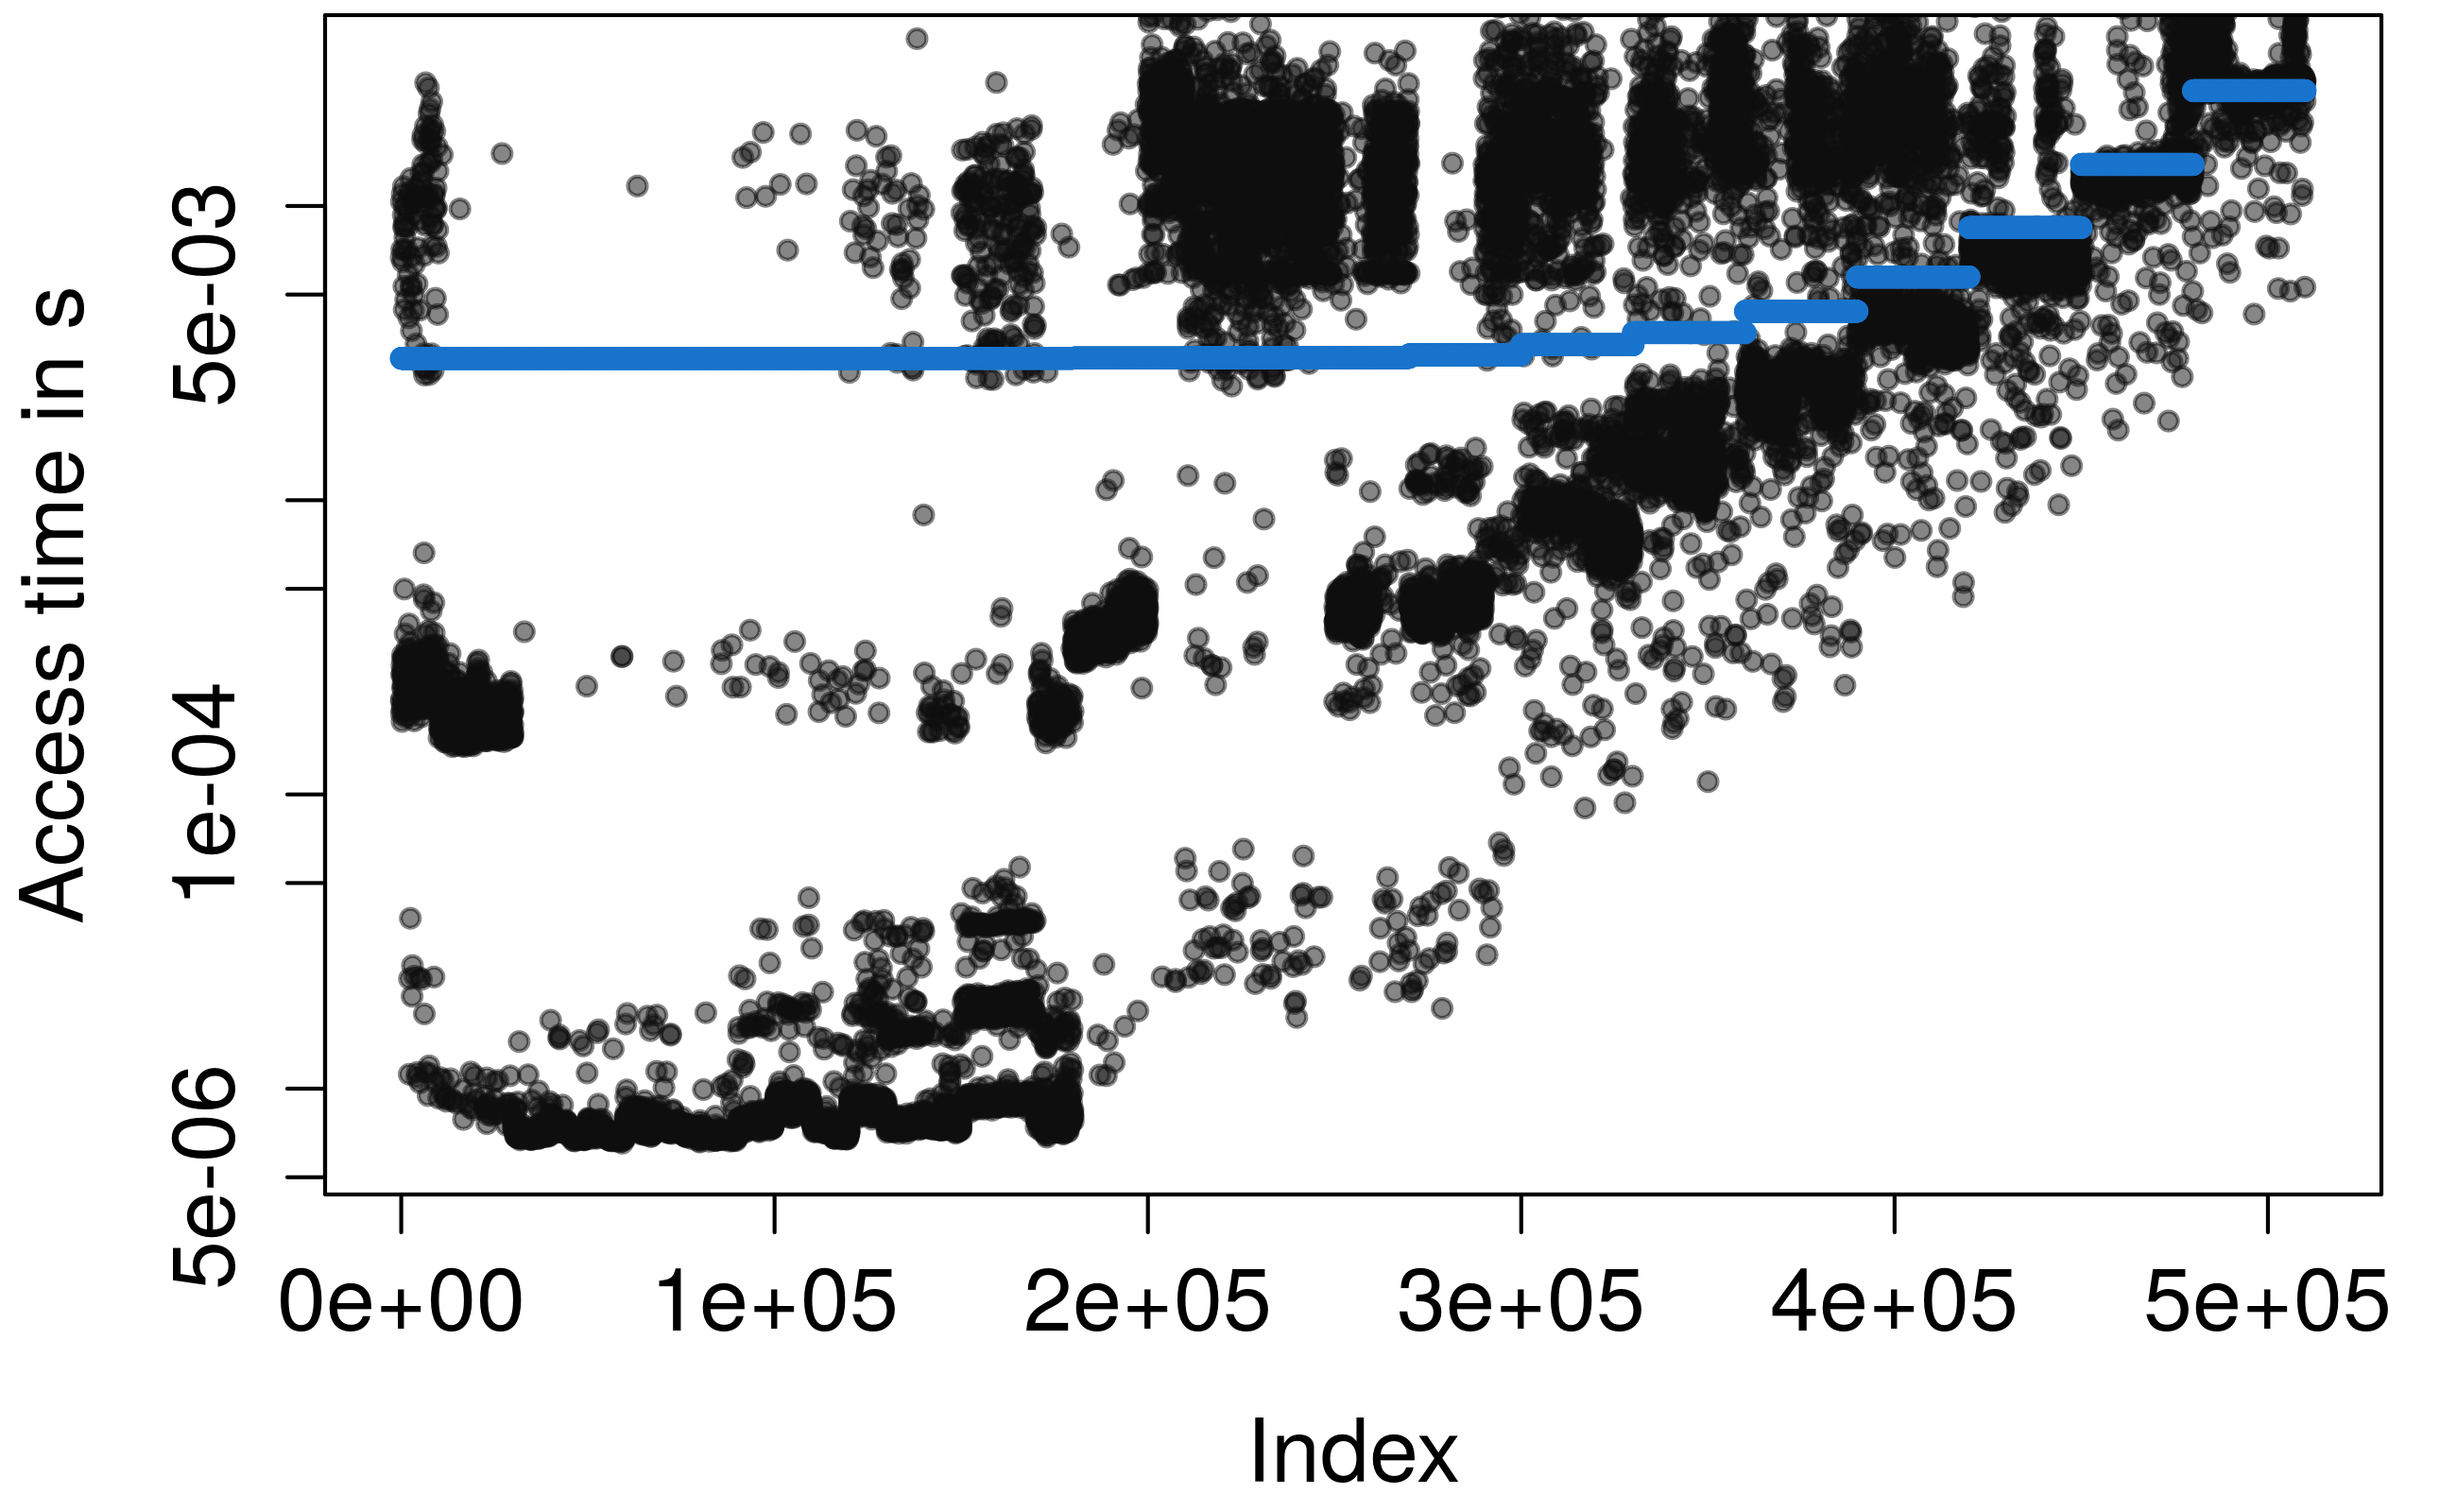
\includegraphics[width=\textwidth]{src/plot_rnd_linreg_Size.png}
		\caption{Predicted access times of the linear regression model as blue points.}
		\label{linreg}
	\end{minipage}
	\hfill
	\begin{minipage}[b]{0.47\textwidth}
		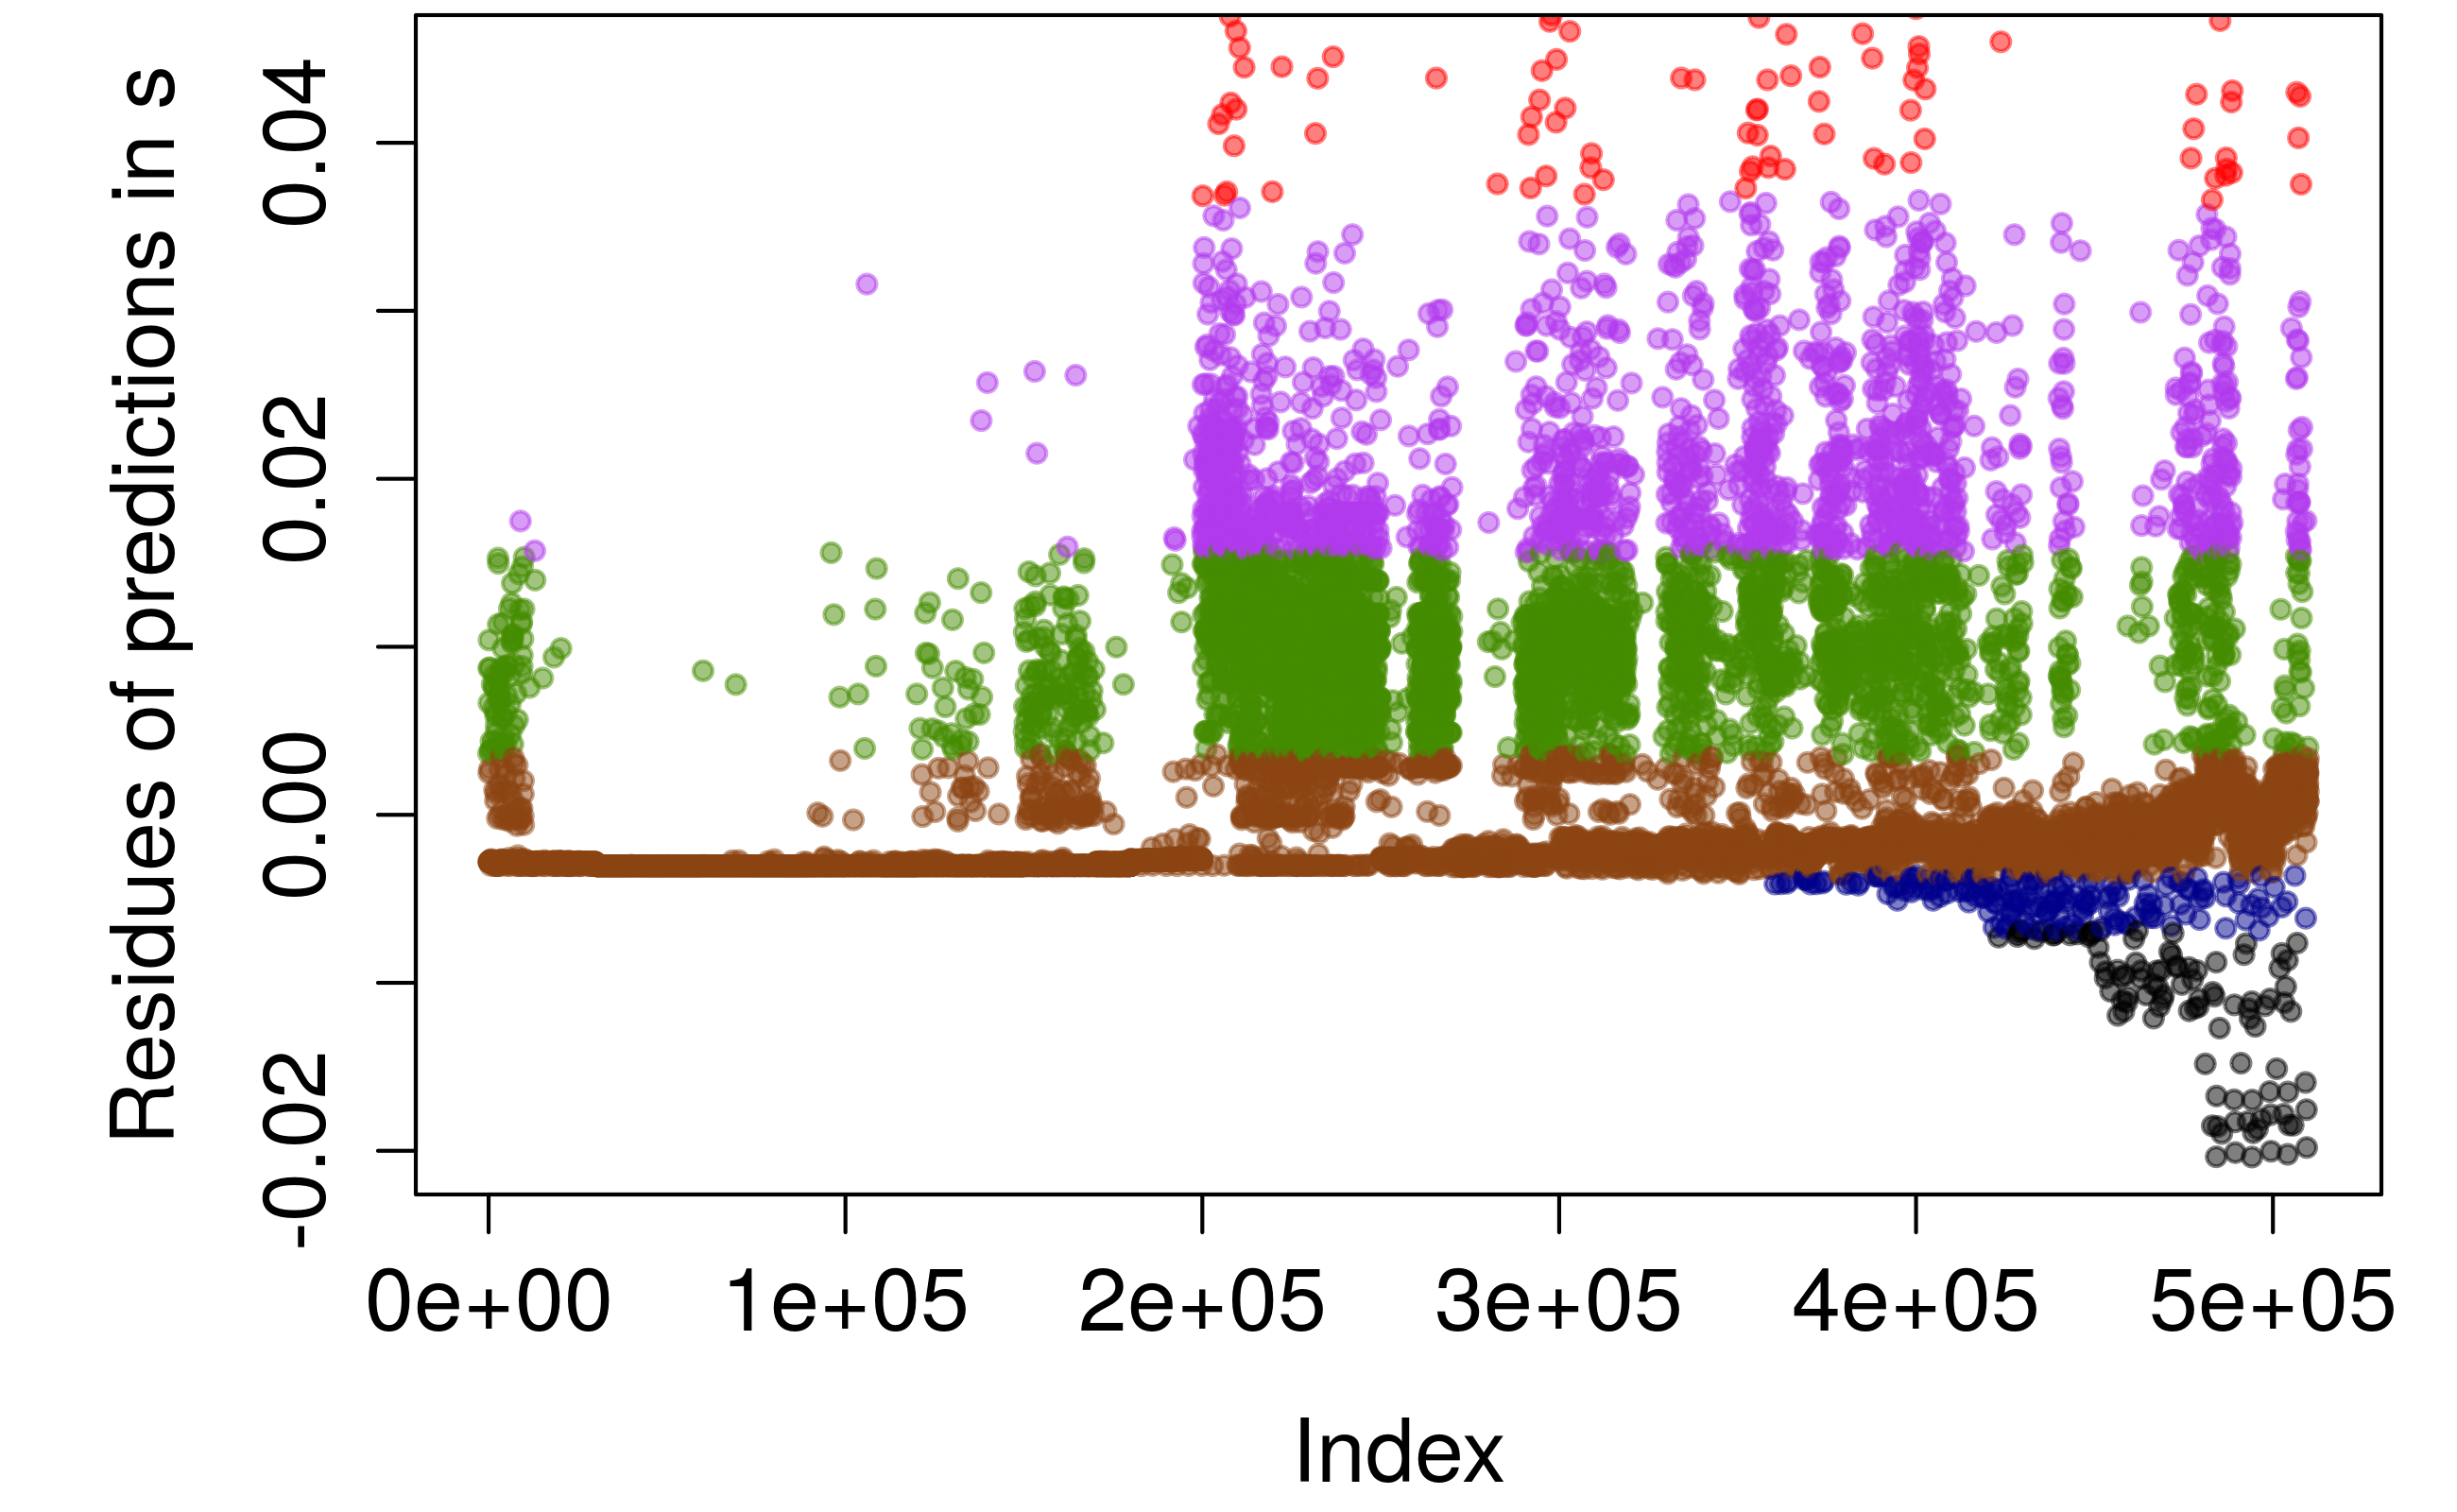
\includegraphics[width=\textwidth]{src/linreg_error_clustering_rnd_all.png}
		\caption{Residues of the linear regression model, colors are corresponding to error classes.}
		\label{clustering}
	\end{minipage}
\end{figure}
%\fig{width=.47\textwidth}{src/plot_rnd_linreg_Size.png}{Predicted access times of the linear regression model as blue points.}
%\fig{width=.47\textwidth}{src/linreg_error_clustering_rnd_all.png}{Residues of the linear regression model, colors are corresponding to error classes.}

For identifying the error classes, the difference between the prediction of linear regression and actual access time is used as input for the clustering algorithm.
In Figure \ref{clustering} the residues for all measurements are shown, the different colors correspond to the computed clusters, which are our error classes. 
Note that due to the random initialization of k-Means, different runs may result in different clusters\,\footnote{We will consider more robust algorithms in the future.}.


The clusters are differentiated along horizontal lines in the graphs.
Without going into further details one can recognize from the graphs already that the error classes are not perfect approximators of I/O-paths.
The measurements with smallest access sizes (on the far left) are only differentiated into two different error classes; however, the two error classes mainly represent  on the one hand measurements with close to 0 or negative error and positive errors on the other hand, what seems to be a reasonable approximation of I/O-paths.\medskip

The computed error classes can be examined in further detail with the data from Table\,\ref{tab:error_classes}.
Ideally for a good correlation of I/O-paths to error classes each error class should represent one particular value of data throughput, which would be characteristic for the slowest storage medium occurring in the I/O-path. 
This is mostly true for the error classes. The classes 4, 5 and 6, however, have with $5.5\cdot10^7$, $6.1\cdot10^7$ and $5.8\cdot10^7$ very similar average throughput values, which might be a hint for too many error classes.\\
\tab{tab:error_classes}{Characteristics of computed error classes for random file accesses in detail.}{
	\centering
	\scriptsize
	\begin{tabular}{|r|r|r|r|r|r|r|r|}\hline%
		& \multicolumn{3}{|c|}{averaged values} & \multicolumn{3}{|c|}{prediction error} & \multicolumn{1}{r|}{} \\ \hline
		Error class & Throughput (B/s) & Access size (B) & Access time (s) & Min (s) & Avg (s) & Max (s) & \# of members\\\hline\hline
		\csvreader[late after line=\\\hline]%
		{src/rnd_linreg_classes_on_seq.csv}{tp=\tp,idx = \idx,rndcount=\rndcount,minerror=\minerror, meanerror = \meanerror, maxerror = \maxerror, seqcount = \seqcount, size = \size, duration = \duration}%
		{\idx & \tp & \size & \duration & \minerror & \meanerror & \maxerror & \rndcount}%
	\end{tabular}
}\\
The vast majority of measurements were assigned to error class 3 which is the error class that covers the range around a prediction error of 0.
Therefore most access times can be predicted sufficiently by the linear regression model.\\
One sign for correct approximation of I/O-paths is it when error classes exist which have equal access sizes but different access times.
In such cases a differentiation of measurements with equal access parameters takes place.
This occurs for example with the error classes 4 and 8. Both classes have an average access size of $1.2\cdot10^6$ Bytes, but with 0.0143 and 0.2741 seconds very different average access times.
The error classes of sequential file accesses are display similar characteristics as the here analyzed random file accesses.

\subsection{Prediction of file accesses}
After we analyzed the benchmarks and error classes we will study the results of our models.
To investigate the accuracy of the models and investigate overfitting, we split the available data into a training set and a test set. 
The test set consist of all measurements that weren't used for training.
The parameters for the ANN-models are varied to explore appropriate configurations; they are trained with a wide span of different parameter values for the number of hidden layers and number of neurons per layer.
They had 1000 randomly chosen measurements for each pair of access size and access type as training set. % TODO stimmt das 1000 pro Konfiguration? Ja, das stimmt :)
In total that are 34\,000 measurements which should be a significant amount of data to avoid a situation in which we aren't able to train a model due to a lack of information about the system. 

\medskip

In Tables\,\ref{tab:seq-stats} and \ref{tab:rnd-stats} characteristics of the ANNs with the smallest average prediction error can be seen.
The models for the sequential data set had in general bigger network structures.
\tab{tab:seq-stats}{Characteristics of the most successful ANN-models for seq. file accesses.}{
	\centering
	\scriptsize
	\begin{tabular}{|r|r|r|r|r|}\hline%
		Model & Hidden layers & Neurons per layer & Computing iterations & Training duration (s) \\\hline\hline
		\csvreader[late after line=\\\hline]%
		{src/latex_seq_net-stats.csv}{Modell=\Model,verdeckteSchichten=\verdeckteSchichten,Neuronen=\Neuronen, Iterationen = \Iterationen, Trainingsdauer = \Trainingsdauer}%
		{\Model & \verdeckteSchichten & \Neuronen & \Iterationen & \Trainingsdauer}%
	\end{tabular}
}
\tab{tab:rnd-stats}{Characteristics of the most succesful ANN-models for random file accesses.}{
	\centering
	\scriptsize
	\begin{tabular}{|r|r|r|r|r|}\hline%
		Model & Hidden layers & Neurons per layer & Computing iterations & Training duration (s) \\\hline\hline
		\csvreader[late after line=\\\hline]%
		{src/latex_rnd_net-stats.csv}{Modell=\Model,verdeckteSchichten=\verdeckteSchichten,Neuronen=\Neuronen, Iterationen = \Iterationen, Trainingsdauer = \Trainingsdauer}%
		{\Model & \verdeckteSchichten & \Neuronen & \Iterationen & \Trainingsdauer}%
	\end{tabular}
}\\
We used the following metrics to quantify the error:
\begin{itemize}
	\item \textbf{MAE}: Mean average error.
	\item \textbf{Avg-MAPE}: The mean absolute percentage error averaged about 12 instances of ANNs with equal parameter values, but different (random) initial network weights.
	\item \textbf{Train-MAPE}: The mean absolute percentage error on the training set. 
	\item \textbf{MAPE}: The mean absolute percentage error (on the test set).
	\item \textbf{MSPE}: Mean squared percentage error.
	\item \textbf{RQ3}: Third quartile of prediction errors, which means that three quarters of the test set were predicted with smaller deviation to the true value that this.
	\item \textbf{PMax}: The biggest prediction error in percent.
\end{itemize}

The prediction errors of our models can be found in the Tables\,\ref{tab:seq-results} and \ref{tab:rnd-results}.
Listed values refer to the model with smallest average prediction error.
We can observe, that for all models values for Avg-MAPE, Train-MAPE and MAPE are close to each other.
This means that the training set was representative for the test set with little overfitting, and also that the model behavior was stable and did not depend so much on the random initiation of network weights.
\tab{tab:seq-results}{Results of our models on the sequential file accesses.}{
	\centering
	\scriptsize
	\begin{tabular}{|p{2.5cm}|r|p{1.4cm}|p{1.4cm}|r|r|r|r|}\hline%
		Model & MAE (s) & Avg- \mbox{MAPE (\%)} & Train- \mbox{MAPE (\%)} &  MAPE (\%) & MSPE (\%) & RQ3 (\%) & PMax (\%) \\\hline\hline
		\csvreader[late after line=\\\hline]%
		{src/latex_seq_results.csv}{Modell=\Model,MAF=\MAF,RMAF=\RMAF, RMQA = \RMQA, Q3 = \Q3, Max = \Max,RMAFTraining = \RMAFTraining, Bereich = \Bereich, RMAFavg = \RMAFavg}%
		{\Model & \MAF & \RMAFavg & \RMAFTraining & \RMAF & \RMQA & \Q3 & \Max }%
	\end{tabular}
}
\tab{tab:rnd-results}{Results of our models on the random file accesses.}{
	\centering
	\scriptsize
	\begin{tabular}{|p{2.5cm}|r|p{1.4cm}|p{1.4cm}|r|r|r|r|}\hline%
		Model & MAE (s) & Avg- \mbox{MAPE (\%)} & Train- \mbox{MAPE (\%)} &  MAPE (\%) & MSPE (\%) & RQ3 (\%) & PMax (\%) \\\hline\hline
		\csvreader[late after line=\\\hline]%
		{src/latex_rnd_results.csv}{Modell=\Model,MAF=\MAF,RMAF=\RMAF, RMQA = \RMQA, Q3 = \Q3, Max = \Max,RMAFTraining = \RMAFTraining, Bereich = \Bereich, RMAFavg = \RMAFavg}%
		{\Model & \MAF & \RMAFavg & \RMAFTraining & \RMAF & \RMQA & \Q3 & \Max}%
	\end{tabular}
}\\
It becomes clear that linear regression is sub-optimal for the prediction of file access times for random file accesses, where it's MAPE is about 5578.4\,\%. For the sequential case the results are better, but still with more than three times higher average percentage error.\medskip

The second thing one can take from the results is that the ema-model did not work as intended.
It's error values are very close to the simple ANN-model which had less input information to work with.
Going a little bit more into detail it is notable that the MAPE is smaller for the ema-models compared to the model without EMA-values.
Thus the additional knowledge was in general useful for better prediction; however, the MSPE and PMax values are higher for the ema-model which means that some predictions were significantly misguided by the EMA-function value.\medskip

In contrast, the error-class-model worked excellent. The mean average error compared with the model without error classes has been reduced to a third for both use cases.
This is a strong confirmation for the thesis that knowledge about I/O-paths is crucial for access time prediction.
However, it is clear that the additional parameter of the error class improves the overall performance of the predictor as we have more input parameters. 

\medskip

To investigate this further, we have to analyze measurements in more detail.
To have a further look at the difference error classes make for access time prediction, we analyze the predictions of the two models for the case of random reading file access in Figure\,\ref{pred_tuple1} and \ref{pred_error}.
\begin{figure}[!h]
	\centering
	\begin{minipage}[b]{0.47\textwidth}
		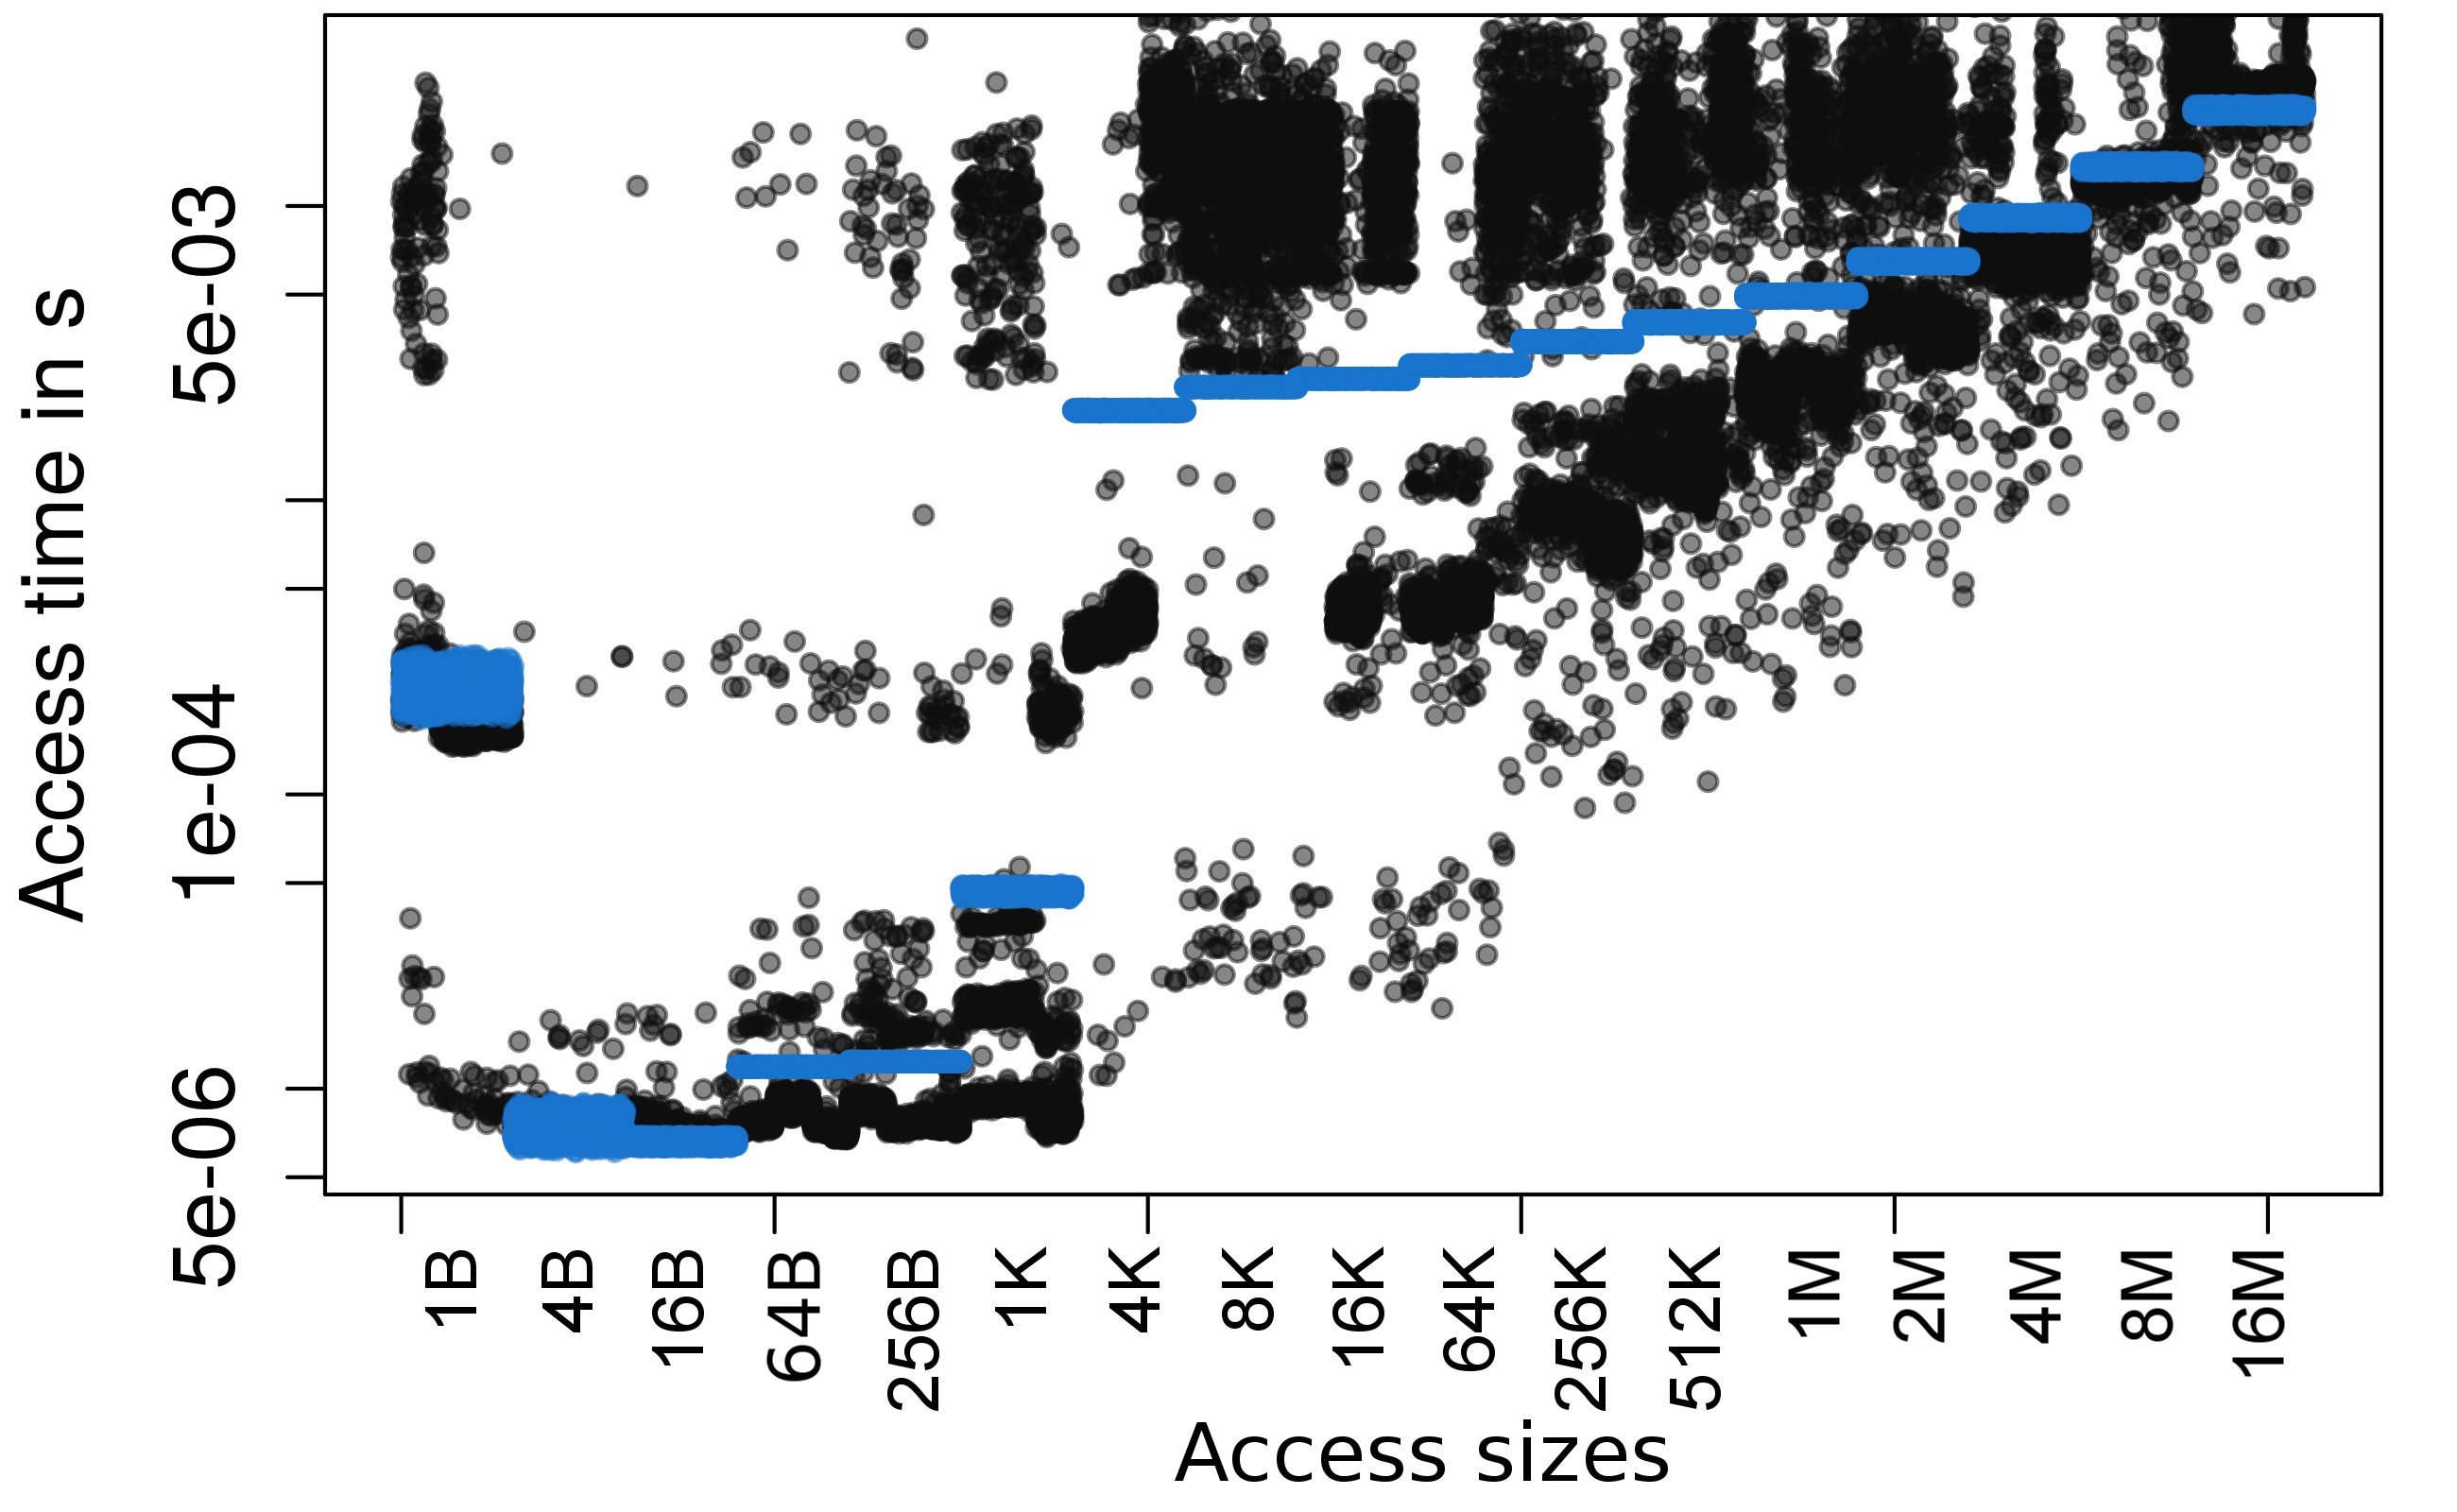
\includegraphics[width=\textwidth]{src/plot_onlyPred_tuple1_Duration_rnd.png}
		\caption{Predicted access times of the simple ANN-model as blue points.}
		\label{pred_tuple1}
	\end{minipage}
	\hfill
	\begin{minipage}[b]{0.47\textwidth}
		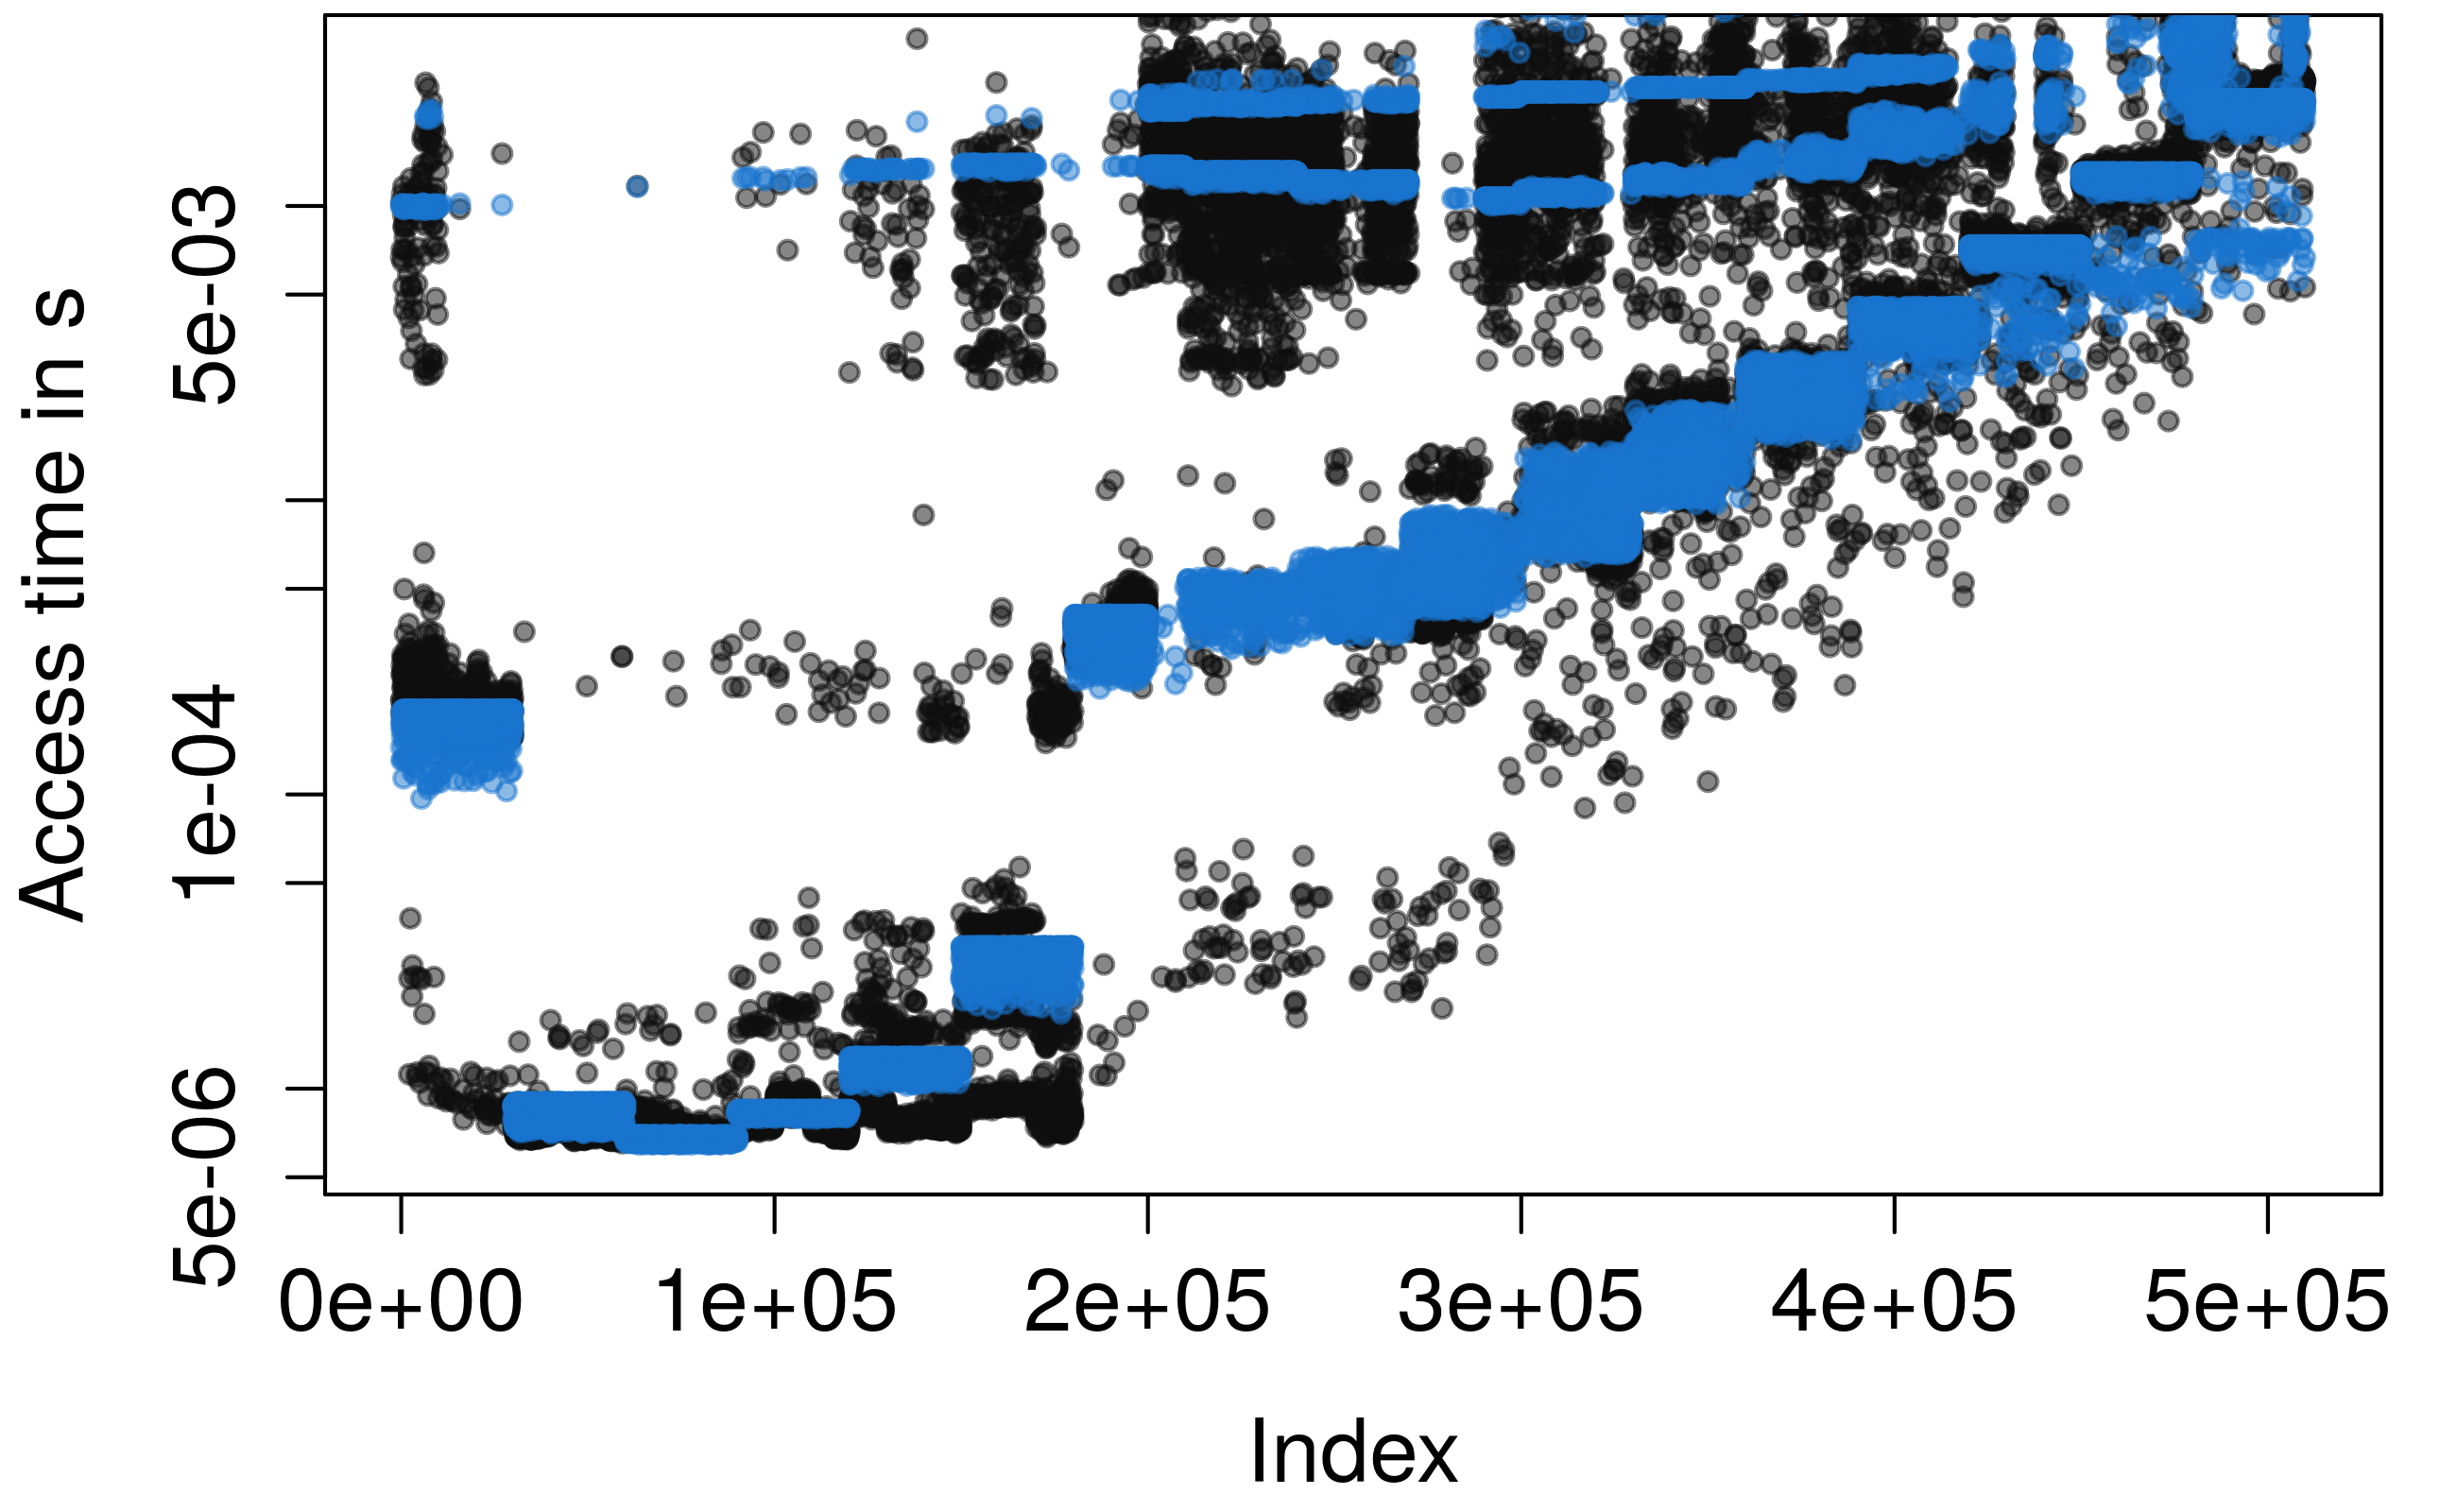
\includegraphics[width=\textwidth]{src/plot_onlyPred_tuple1_with_error_class_from_linreg_Duration_rnd.png}
		\caption{Predicted access times of the error-class-model as blue points..}
		\label{pred_error}
	\end{minipage}
\end{figure}
%\fig{width=.47\textwidth}{src/plot_onlyPred_tuple1_Duration_rnd.png}{Predicted access times of the simple ANN-model as blue points.}\\
%\fig{width=.47\textwidth}{src/plot_onlyPred_tuple1_with_error_class_from_linreg_Duration_rnd.png}{Predicted access times of the error-class-model as blue points.}\\
The model without knowledge about I/O-paths is forced to predict some kind of average access time for each set of measurements with equal access parameter values, therefore its predictions are in between the two main groups of access time for the higher access sizes.
With knowledge about our approximations of I/O-paths the error-class-model can discriminate measurements with equal access parameter values and achieve more accurate predictions that way.

\section{Conclusion and future work}
\label{conclusion}
In this work, we analyzed the performance of a supercomputer's storage system.
Using a machine learning approach with artificial neural networks, we developed different models for file access time prediction.
Through our study of measured file access times and model results we were able to gain knowledge about the behavior of the storage system.
We found out that linear models are not feasible for access time prediction, despite the strong correlation of access time to access size.
Our models utilizing ANNs achieved much better results than linear regression.\\
The hypothesis that knowledge about the internal processing of a file access in form of I/O-paths is essential for access time prediction was supported by our data.
This is because file accesses with equal access parameters can produce strongly deviating access times depending on the used I/O-path.\\
Our approach of deriving knowledge about I/O-paths by exploiting periodic performance of the storage system was not successful.
The additional input information did not lead to a significant improvement of access time predictions.\\
However, with our method of clustering residues of linear regression for approximations of I/O-paths as error classes, we were able to illustrate the importance of I/O-paths for access time prediction. The ANN-model with additional input information of error classes was able to reduce its average prediction error to a third compared to the ANN-model with only access parameter values as input information.\medskip

For future work a more elaborate approach for exploitation of the periodic storage performance could be used. 
Crume et al. had success on access time prediction for single hard drives using Fourier analysis \cite{Crume:2013:FML:2538542.2538561} or additional sinusoids as input for ANNs \cite{crumelatent}.\\
Secondly the error path method could be researched in further detail.
Residues of other models than linear regression could be used and one could try to assign error classes to I/O-paths in a real system -- the administrator would have to investigate the error classes and define them according to the storage technology.
The method could also be a starting point to develop a tool that provides information on the effectiveness of the used I/O during execution of a program.

%\ack{Put the acknowledgements after the last section, like this.}
\openaccess

\bibliography{literatur}

%\received{September 25, 2013}

\end{document}
